\documentclass[11pt]{article}

\usepackage{
    amssymb,
    amsmath,
    amsfonts,
    calc,
    eurosym,
    geometry,
    ulem,
    graphicx,
    caption,
    color,
    setspace,
    sectsty,
    comment,
    footmisc,
    caption,
    % natbib,
    pdflscape,
    subcaption,
    subfiles,
    titling,
    array,
    hyperref,
    booktabs,
    longtable,
    float,
    authblk,
    makecell,
    threeparttable}


\usepackage[
    backend=biber,
    style=nature,
    date=year,
    doi=true,
    isbn=false,
    url=false,
    eprint=false
]{biblatex}

\AtEveryBibitem{%
  \clearfield{note}%
}
\AtEveryCitekey{\clearlist{publisher}}
\AtEveryBibitem{\clearlist{publisher}}

\usepackage{pgf,tikz}
\usetikzlibrary{arrows, automata}
\usetikzlibrary{shapes.geometric,positioning}
\usetikzlibrary{positioning,calc}

\usepackage{siunitx}
\newcolumntype{d}{S[input-symbols = ()]}

\normalem

\renewcommand\Affilfont{\small\itshape}

\onehalfspacing
\newtheorem{theorem}{Theorem}
\newtheorem{corollary}[theorem]{Corollary}
\newtheorem{proposition}{Proposition}
\newtheorem{definition}{Definition}

\newenvironment{proof}[1][Proof]{\noindent\textbf{#1.} }{\ \rule{0.5em}{0.5em}}

\newtheorem{hyp}{Hypothesis}
\newtheorem{subhyp}{Hypothesis}[hyp]
\renewcommand{\thesubhyp}{\thehyp\alph{subhyp}}

\newcommand{\red}[1]{{\color{red} #1}}
\newcommand{\blue}[1]{{\color{blue} #1}}

\newcolumntype{L}[1]{>{\raggedright\arraybackslash}m{#1}}
\newcolumntype{C}[1]{>{\centering\arraybackslash}m{#1}}
\newcolumntype{R}[1]{>{\raggedleft\arraybackslash}m{#1}}
\subsubsectionfont{\normalfont\itshape}

\usepackage{mathtools}

\usepackage{letltxmacro}
\LetLtxMacro\orgvdots\vdots
\LetLtxMacro\orgddots\ddots

\makeatletter
\DeclareRobustCommand\vdots{%
  \mathpalette\@vdots{}%
}
\newcommand*{\@vdots}[2]{%
  % #1: math style
  % #2: unused
  \sbox0{$#1\cdotp\cdotp\cdotp\m@th$}%
  \sbox2{$#1.\m@th$}%
  \vbox{%
    \dimen@=\wd0 %
    \advance\dimen@ -3\ht2 %
    \kern.5\dimen@
    % remove side bearings
    \dimen@=\wd2 %
    \advance\dimen@ -\ht2 %
    \dimen2=\wd0 %
    \advance\dimen2 -\dimen@
    \vbox to \dimen2{%
      \offinterlineskip
      \copy2 \vfill\copy2 \vfill\copy2 %
    }%
  }%
}
\DeclareRobustCommand\ddots{%
  \mathinner{%
    \mathpalette\@ddots{}%
    \mkern\thinmuskip
  }%
}
\newcommand*{\@ddots}[2]{%
  % #1: math style
  % #2: unused
  \sbox0{$#1\cdotp\cdotp\cdotp\m@th$}%
  \sbox2{$#1.\m@th$}%
  \vbox{%
    \dimen@=\wd0 %
    \advance\dimen@ -3\ht2 %
    \kern.5\dimen@
    % remove side bearings
    \dimen@=\wd2 %
    \advance\dimen@ -\ht2 %
    \dimen2=\wd0 %
    \advance\dimen2 -\dimen@
    \vbox to \dimen2{%
      \offinterlineskip
      \hbox{$#1\mathpunct{.}\m@th$}%
      \vfill
      \hbox{$#1\mathpunct{\kern\wd2}\mathpunct{.}\m@th$}%
      \vfill
      \hbox{$#1\mathpunct{\kern\wd2}\mathpunct{\kern\wd2}\mathpunct{.}\m@th$}%
    }%
  }%
}
\makeatother


\newcommand{\ode}[2]{\frac{d{#1}}{d{#2}}}
\DeclareMathOperator{\E}{E}
\DeclareMathOperator{\indep}{\perp\!\!\!\perp}
\geometry{left=1.0in,right=1.0in,top=1.0in,bottom=1.0in}

\addbibresource{tnd.bib}

\begin{document}
%TC:ignore
\begin{titlepage}
\title{Identifying vaccine effectiveness in the test-negative design under an equi-confounding assumption}
\author[1]{Christopher Boyer}%\thanks{email: \href{mailto:cboyer@hsph.harvard.edu}{cboyer@hsph.harvard.edu}}}
\author[2]{Kendrick Qijun Li}
\affil[1]{Department of Epidemiology, Harvard T.H. Chan School of Public Health, Boston, MA.}
\affil[2]{Department of Biostatistics, St. Jude Children's Research Hospital, Memphis, TN.}
\date{\today\vspace{-1em}}
\maketitle

\begin{abstract}
    The test-negative design (TND) is frequently used to evaluate vaccine effectiveness in real-world settings. In a TND study, individuals with similar symptoms who seek care are tested for the disease of interest, and effectiveness is estimated by comparing the vaccination history of test-positive cases and test-negative controls. Traditional approaches justify the TND by assuming either (a) receiving a test is a perfect proxy for unmeasured health-seeking behavior or (b) vaccination is unconfounded given measured covariates ---both of which may be unrealistic. In this paper, we return to the original motivation for the TND and propose an alternative justification based on the assumption of \textit{odds ratio equi-confounding}, where unmeasured confounders influence test-positive and test-negative individuals equivalently on the odds ratio scale. We discuss the implications of this assumption for TND design and provide alternative estimators for the marginal risk ratio among the vaccinated, using outcome modeling, inverse probability weighting, and an efficient influence function to accommodate flexible machine learning models. We present proofs of our results and conduct a simulation study to evaluate the empirical performance of these estimators when our assumptions hold and when they are violated.

\noindent \\
\noindent\textbf{Keywords:} test-negative design, vaccine effectiveness, causal inference, observational studies, unmeasured confounding, equi-confounding, odds ratios, selection bias
\bigskip
\end{abstract}
\setcounter{page}{0}
\thispagestyle{empty}
\end{titlepage}
\pagebreak \newpage
%TC:endignore

%\doublespacing

\section{Introduction} \label{sec:introduction}
Post-market evaluation of vaccine effectiveness is critical for understanding how vaccines perform in real-world settings \cite{patel_postlicensure_2020}. As population immunity changes and pathogens undergo antigenic mutation or selection, pre-market randomized trial estimates may lose relevance over time \cite{hitchings_effectiveness_2021,israel_elapsed_2021}. Investigators may also want to evaluate vaccine performance in certain subpopulations that were either ineligible or underrepresented \cite{olson_effectiveness_2022}, assess outcomes and safety signals that may have been underpowered \cite{thompson_effectiveness_2021}, or compare vaccine formulations head-to-head or against other therapeutics not considered in the original trials \cite{skowronski_two-dose_2022}. Often, these evaluations must rely on observational data \cite{chua_use_2020-1,dean_covid-19_2021}. Under these circumstances, the test-negative design (TND) is a cost-effective and efficient study design for estimating vaccine effectiveness \cite{sullivan_potential_2014,jackson_test-negative_2013}. 
 
In the literature, the term ``test-negative design'' has sometimes been applied loosely to any study where individuals who test positive for a disease of interest are compared with those who test negative. However, not all such studies are methodologically equivalent. Here, we focus on the canonical design with the following criteria: patients with acute respiratory illness are prospectively recruited using a unified symptom screen through hospitals or other care facilities, consented, and a laboratory test for the pathogen of interest is performed. Detailed information about their demographic, medical, and vaccination history is collected via a questionnaire at enrollment or through linked medical and vaccination records. Those who test positive form the ``cases'' and those who test negative are the ``controls''. Vaccine effectiveness is then estimated via the case status odds ratio among those screened and tested.

This version of the TND has been previously championed on the grounds that it is robust to unmeasured confounding by healthcare-seeking behavior  --- a common source of bias in observational evaluations of vaccines and in particular seasonal influenza vaccines \cite{jackson_test-negative_2013}. Because participants seek a test conditional on the same symptom set but without knowledge of the causative agent, it was claimed the design effectively restricts to care-seekers, thereby precluding it as potential confounder \cite{jackson_test-negative_2013}. It was also suggested that, by limiting to individuals who actually received a test, the TND may be less subject to measurement error \cite{jackson_test-negative_2013}. Subsequent work pointed out that the TND (i) is subject to residual confounding when healthcare-seeking is nonbinary or when there are other factors affecting vaccine uptake and risk of infection \cite{sullivan_theoretical_2016,lewnard_theoretical_2021,lipsitch_observational_2016}, (ii) is subject to possible selection bias due to conditioning on the post exposure outcome of receiving a test \cite{sullivan_theoretical_2016,lipsitch_observational_2016}, and (iii) is biased when vaccination has a direct effect on testing behavior \cite{foppa_case_2013}. 

More recently, \textcite{schnitzer_estimands_2022} introduced a formal causal framework for the TND based on potential outcomes, allowing for a more precise discussion of causal identification in the TND. In follow up work, they showed that both the marginal and conditional causal risk ratios can be identified using data from a TND and suggest efficient estimators, but require that observed covariates are sufficient to ensure no unmeasured confounding or selection bias \cite{jiang_tnddr_2023}. However, this assumption is contrary to the original motivation for the TND. Thus, a question remains as to whether the TND may be formally justified under weaker assumptions.

In this article, we return to the original motivation and show that the TND may be justified under an alternative assumption that unmeasured confounding is equivalent for test-positive cases and test-negative controls on the odds ratio scale. This assumption builds on the insight that infection with another respiratory illness, if unaffected by focal vaccination, is effectively a negative outcome control \cite{lipsitch_negative_2010,shi_selective_2020}. Therefore any observed differences in the incidence of test negative illnesses between vaccinated and unvaccinated individuals likely reflect residual confounding. Under the strong assumption of confounding equivalence, we can then use the difference in test-negative illness to de-bias our estimate of vaccine effectiveness, similar to the parallel trends concept in the difference-in-differences literature \cite{sofer_negative_2016,park_universal_2023,tchetgen_universal_2023}. As we show, this approach remains valid under the outcome-dependent sampling of the TND, where only those who are tested are sampled, if we further assume that (potentially unobserved) determinants of care-seeking behavior are equivalent for test-positive and test-negative illnesses, which could be justified given the causative agent is unknown to individuals prior to receiving a test.  When our assumptions hold, we show that the traditional odds ratio estimator from the TND identifies the conditional risk ratio \textit{among the vaccinated} in the population. We also derive new estimators of the marginal risk ratio among the vaccinated, including those based on outcome modeling and inverse probability weighting. We discuss the implications of our assumptions for the design of TNDs and provide proofs of our results as well as simulations to illustrate the consequences when our assumptions are violated.

\section{Setup and observed data} \label{sec:setup}
Let $X$ represent a vector of baseline (pre-vaccination) covariates, $V$ an indicator of vaccination status, and $I$ a categorical indicator of symptomatic illness where
        $$I := \begin{cases} 
        I = 2 & \text{when symptomatic illness is caused by the pathogen of interest}, \\
        I = 1 & \text{when symptomatic illness is caused by something else}, \\
        I = 0 & \text{when no symptomatic illness}.
        \end{cases}$$
 Implicit here is the assumption that the infection events represented by $I = 1$ and $I = 2$ are mutually exclusive. For convenience, throughout we use the term ``symptomatic'' illness to mean the presence of the pre-specified symptom set used to screen for inclusion in the TND study. Let $T$ be an indicator of receiving a test for the pathogen of interest (1: tested, 0: not tested), and $I^*$ the result of the test (1: positive, 0: negative). For now, assume that the test is perfect, such that for all individuals, $I^*_i = \mathbbm{1}(I_i = 2, T_i = 1)$, where $\mathbbm{1}(\cdot)$ is the indicator function. Extensions to cases where the test is imperfect are covered in Appendix \ref{sec:testing} but also have been considered previously \cite{jackson2015effects, sullivan_theoretical_2016}. Throughout we denote by $I^v$ the potential outcome under an intervention that sets vaccination to $V=v$. 
    
We assume the data from the TND are independent realizations of 
$$O = \{(X_i, V_i, S_i = 1, I^*_i) : i = 1, \ldots, n\}$$
where $S$ is an indicator of selection into test-negative design under potentially biased sampling from the underlying target population. Selection is minimally based on presenting with a set of pre-specified symptoms at a health facility and receiving a test, i.e. $S = \mathbbm{1}(I \neq 0, T = 1)$, but could be extended to include other criteria such as hospitalization or severe disease. We assume that the symptom screen is effective such that everyone tested has either $I=1$ or $I=2$. Vaccination status and associated covariates may be retrospectively assessed at the time of testing or, preferably, pulled from outside sources such as vaccine registries or healthcare databases. 

\section{Causal estimands for the test-negative design} \label{sec:estimands}
In a TND study, a common target parameter is the causal risk ratio,
\begin{equation*}
    \Psi_{RR} \equiv \dfrac{\Pr[I^1 = 2, T^1 = 1]}{\Pr[I^0 = 2, T^0 = 1]},
\end{equation*}
which contrasts the joint probability of symptomatic infection and receipt of a test (i.e. seeking medical care) in the population underlying the TND if everyone were vaccinated compared to if they were unvaccinated, with \textit{vaccine effectiveness} defined as $1 - \Psi_{RR}$. In some cases, the causal odds ratio is the focus instead of the risk ratio, although this is often combined with an assumption ---either explicit or implicit--- that symptomatic infection is rare in the population underlying the TND over the follow up period, in which case the odds ratio approximates the risk ratio. Following the literature, we refer to the joint outcome $\mathbbm{1}(I^1 = 2, T^1 = 1)$ as \textit{medically-attended illness}, presuming that inclusion in the TND necessitates symptomatic infection severe enough to require medical care. 

Under the assumption that the measured covariates, $X$, are sufficient to control confounding and selection bias, \Citeauthor*{schnitzer_estimands_2022} \cite{schnitzer_estimands_2022} showed that the odds ratio comparing vaccination among test-positive cases and test-negative controls under the biased sampling of the test-negative design is a consistent estimator of $\Psi_{RR}$. Here, we relax the no unmeasured confounding assumption. However, this requires that we focus instead on the causal risk ratio \textit{among the vaccinated}, i.e.
\begin{equation*}
    \Psi_{RRV} \equiv \dfrac{\Pr[I^1 = 2, T^1 =1 | V = 1]}{\Pr[I^0 = 2, T^0 =1 | V = 1]} .
\end{equation*}
rather than the risk ratio in the full population. This parameter is analogous to the average treatment effect on the treated (ATT) in the causal inference literature, though expressed as a ratio rather than a difference. When vaccination provides constant protection for everyone, $\Psi_{RRV}$ will coincide with the causal risk ratio in the full population, i.e. $\Psi_{RR} = \Psi_{RRV}$. However, when protection is heterogeneous, the causal risk ratio in the full population becomes a weighted average of the causal risk ratio among the vaccinated and unvaccinated.

% When there is no direct effect of vaccination on testing (formalized below), then $\Psi_{RR}$ is equivalent to the causal risk ratio for \textit{testing positive} with symptomatic illness,
% \begin{equation*}
%     \Psi_{RR} = \dfrac{\Pr[I^1 = 2, T^1 = 1]}{\Pr[I^0 = 2, T^0 = 1]}.
% \end{equation*}
% Note, this would be true, for instance, in a double-blind placebo-controlled randomized trial in which participants present naturally for testing when they develop symptoms rather than being randomly sampled and tested regardless of symptoms on a given follow up day. In previous work, the joint outcome is sometimes referred to as medically-attended illness \cite{jackson_test-negative_2013}, under the presumption that to receive a test requires sufficiently acute disease to warrant seeking care. 

\section{Identification} \label{sec:identification}
\subsection{Identifiability conditions} \label{sec:conditions}
    To identify the causal risk ratio among the vaccinated, $\Psi_{RRV}$, we rely on the following conditions
\begin{enumerate}[label=\upshape(A\arabic*), ref=A\arabic*]
    \item\label{ass1} \textit{Consistency of potential outcomes}. For all individuals $i$ and for $v \in \{0, 1\}$, we have $I_i^v = I_i$ and $T_i^v = T_i$ when $V_i = v$. 
    \item\label{ass2} \textit{No effect of vaccination on testing negative and symptomatic among the vaccinated}. That is, $\Pr[I^0 = 1, T^0=1 | V = 1, X] = \Pr[I^1 = 1, T^1=1 | V = 1, X].$
    \item\label{ass3} \textit{Odds ratio equi-confounding}. Degree of unmeasured confounding bias on the odds ratio scale is the same for test-positive and test-negative illnesses, i.e. 
    $$OR_2(X) = OR_1(X), $$
    $$ \text{where } OR_i(X) = \frac{\Pr[I^0 = i, T^0 = 1 | V = 1, X]\Pr[T^0 = 0 | V = 0, X]}{\Pr[T^0 = 0 | V = 1, X]\Pr[I^0 = i, T^0 = 1| V = 0, X]}.$$
    \item\label{ass4} \textit{Overlap of vaccination among test-positives and test-negatives}. Define $\mathcal{S}_i(v)$ as the support of the law of $(I^0 = i, T^0 = 1, V = v, X)$, then for $v$ in $\{0,1\}$, then it must be that $\mathcal{S}_2(1) \subseteq \mathcal{S}_2(0)$ and $\mathcal{S}_2(v) \subseteq \mathcal{S}_1(v).$
    %\item[(A5)] No direct effect of vaccination on test-seeking behavior among the vaccinated. That is, for $i$ in $\{1,2\}$, $\Pr[T^1 = 1 | I^1 = i, V = 1, X] = \Pr[T^0 = 1 | I^0 = i, V = 1, X].$
\end{enumerate}

Assumption \ref{ass1} is a well-known identifiability condition in the causal inference literature discussed in more detail elsewhere \cite{hernan_causal_2020}. Assumption \ref{ass2} has two implications. First, it implies that the vaccine does not offer any cross-protection against other types of infection which may cause the same symptoms, including any short-term, nonspecific protection via activation of the immune system. Second, it requires that an individual's decision to seek care and get tested is unaffected by their vaccination status, though it may depend on other measured and unmeasured factors. In theory, \ref{ass2} could be evaluated in a randomized trial by comparing the incidence of testing negative (or testing positive for specific non-target pathogens) across the vaccine and comparison arms. However, in practice, trials may not be adequately powered to rule out small effects. In placebo-controlled trials, differences in care-seeking are minimized through the blinding of the participant to their vaccination status. Both aspects of \ref{ass2} have been invoked in previous TND studies \cite{jackson_test-negative_2013,feng_assessment_2017,schnitzer_estimands_2022}. In Appendix \ref{sec:de_testing}, we show that assumption \ref{ass2} can be further relaxed if the effect of vaccination on testing is equivalent for test-positive and test-negative illnesses.

Assumption \ref{ass3} is the key assumption of this paper and offers an alternative to the strict no unmeasured confounding (i.e. conditional independence) assumption suggested previously \cite{schnitzer_estimands_2022}. It states that the degree of unmeasured confounding on the odds ratio scale is the same for test-positive and test-negative illnesses. Notably, it does not require unmeasured confounders to be binary or even related to health-seeking specifically, although health-seeking behavior is certainly a credible candidate for satisfying this condition. \citeauthor{lewnard_measurement_2018} briefly mentioned a similar condition, although not in a formal causal framework \cite{lewnard_measurement_2018}. The assumption is also similar to a recently suggested scale-independent alternative to the parallel trend assumption in the difference-in-differences literature \cite{park_universal_2023,tchetgen_universal_2023}. We discuss the underlying parameterization in more detail in Appendix \ref{sec:or_model}. When $I = 1$ and $I = 2$ are mutually exclusive, assumption  \ref{ass3} simplifies to
\begin{equation}\label{eqn:a3_simplified}
    \frac{\Pr[I^0 = 2, T^0 = 1 | V = 1, X]}{\Pr[I^0 = 2, T^0 = 1 | V = 0, X]} =\frac{\Pr[I^0 = 1, T^0 = 1 | V = 1, X]}{\Pr[I^0 = 1, T^0 = 1 | V = 0, X]}.
\end{equation}
Further, by factorizing, we can split \ref{ass3} into two parts, emphasizing the dual influences of confounding and selection:
\begin{enumerate}[label=\upshape(A3\alph*), ref=A3\alph*]
    \item\label{ass3a}  \textit{Odds ratio equi-confounding}. Degree of unmeasured confounding bias on the odds ratio scale is the same for symptomatic illness regardless if $I=1$ or $I=2$ is cause, i.e. 
    $$\frac{\Pr[I^0 = 2 | V = 1, X]}{\Pr[I^0 = 2 | V = 0, X]} =\frac{\Pr[I^0 = 1 | V = 1, X]}{\Pr[I^0 = 1 | V = 0, X]}.$$
    \item\label{ass3b} \textit{Odds ratio equi-selection}. Degree of unmeasured selection bias, e.g. receiving a test, on the odds ratio scale is the same for all symptomatic illness regardless if $I=1$ or $I=2$ is cause, i.e. 
    $$\frac{\Pr[T^0 = 1 | I^0 = 2, V = 1, X]}{\Pr[T^0 = 1 | I^0 = 2, V = 0, X]} =\frac{\Pr[T^0 = 1 | I^0 = 1, V = 1, X]}{\Pr[T^0 = 1 | I^0 = 1, V = 0, X]}.$$
\end{enumerate}
Assumptions \ref{ass3a} and \ref{ass3b} are stronger than \ref{ass3} alone as \ref{ass3} allows, in principle, for situations in which the factored terms in \ref{ass3a} and \ref{ass3b} are both unequal but they cancel when multiplied such that \ref{ass3} still holds. However, whether such a mechanism is likely to occur in practice is doubtful.

Finally, Assumption \ref{ass4} is similar to, although less restrictive than, the well-known positivity condition in causal inference \cite{hernan_causal_2020}. Specifically, \ref{ass4} requires overlap of vaccination propensity between the observed vaccinated and unvaccinated among the test positive cases as well as overlap of vaccination propensity across test-positive cases and test-negative controls within observed vaccination groups. Taken together, the conditions $\mathcal{S}_2(1) \subseteq \mathcal{S}_2(0)$ and $\mathcal{S}_2(v) \subseteq \mathcal{S}_1(v)$ ensure that the odds ratios $OR_2(X)$ and $OR_1(X)$ are well-defined (i.e. nonzero in numerator and denominator).

% \subsection{Graphical criteria} \label{sec:graphical}
The causal directed acyclic graphs (DAGs) in Figure \ref{fig:dags} illustrate possible data generating mechanisms underlying the TND. In these graphs, we introduce $U$, representing a potential unmeasured confounder, to the previous setup. Figures \ref{fig:dag_a} and \ref{fig:dag_b} show mechanisms discussed previously in the TND literature. Figure \ref{fig:dag_a} is a modified version of the DAG in \citeauthor{schnitzer_estimands_2022} \cite{schnitzer_estimands_2022}, where the lack of an arrow from $U$ to $V$ indicates no unmeasured confounding or selection bias. Assumption \ref{ass2} is also shown by the lack of a direct arrow from $V$ to $T$, implying no direct effect of vaccination on testing behavior. Figure \ref{fig:dag_b} is a modified version of the DAG in \citeauthor{sullivan_theoretical_2016} \cite{sullivan_theoretical_2016}, where $U$ is binary health seeking behavior that is synonymous with receiving a test and therefore effectively conditioned on by conditioning on testing.  

The DAG in Figure \ref{fig:dag_c} shows a possible mechanism satisfying the identifiability conditions in this study. It includes the possibility of unmeasured confounding and selection bias, as there is now an arrow from $U$ to $V$; however, as shown by the bold arrows, $U$ is assumed to act equivalently, on the odds scale, for the test positive and test negative illnesses. This condition imposes a parametric restriction on the allowable data generation mechanisms implied by the DAG and as such requires nonstandard notation. The DAGs in Figures \ref{fig:dag_d} and \ref{fig:dag_e} depict alternative mechanisms in which only equi-confounding, Assumption \ref{ass3a}, or equi-selection, Assumption \ref{ass3b}, are assumed. In Figure \ref{fig:dag_split}, we show an alternative DAG that splits the $I$ node into $I_1 = \mathbbm{1}(I = 1)$ and $I_2 = \mathbbm{1}(I = 2)$ with the dashed arrow between them representing the deterministic relationship as they are assumed to be mutually exclusive. This graph allows us to show Assumption \ref{ass2} by the lack of a directed arrow between $V$ and $I_1$. 

\subsection{The test-negative illness as a proxy for unmeasured confounding} \label{sec:effect_among_vaccinated}
To build intuition about the role of conditions \ref{ass1} - \ref{ass4}, consider briefly the identification of the \textit{conditional} causal risk ratio among the vaccinated, i.e.
\begin{equation*}
    \Psi_{RRV}(X) \equiv \frac{\Pr[I^1 = 2, T^1 = 1 | V = 1, X]}{\Pr[I^0 = 2, T^0 = 1 | V = 1, X]}.
\end{equation*}
Multiplying by one in the form of $\frac{\Pr[I^0 = 2, T^0 = 1| V = 0, X]}{\Pr[I^0 = 2, T^0 = 1 | V = 0, X]}$ and applying consistency (Assumption \ref{ass1}), we can decompose $\Psi_{RRV}(X)$ as follows:
\begin{align} \label{eqn:decomposition}
    \Psi_{RRV}(X) &=\underbrace{\frac{\Pr[I = 2, T = 1 | V = 1, X]}{\Pr[I = 2, T = 1 | V = 0, X]}}_{\text{observed risk ratio}} \times \underbrace{\frac{\Pr[I^0 = 2, T^0 = 1 | V = 0, X]}{\Pr[I^0 = 2, T^0 = 1 | V = 1, X]}}_{\text{de-biasing term}}.
\end{align}
This equation shows $\Psi_{RRV}(X)$ can be written as the product of two terms: the (crude) observed risk ratio and a de-biasing term. The de-biasing term represents the ratio of the potential outcomes if vaccination were withheld between those who were, in fact, vaccinated and those who were not. When there is no unmeasured confounding, the de-biasing term equals one and the observed risk ratio equals the causal risk ratio among the vaccinated. Conversely, in the presence of unmeasured confounding, the de-biasing term is the quantity necessary to remove bias from the observed risk ratio. However, without additional assumptions, this term cannot be identified from the observed data. 

One approach is to find a proxy for $\frac{\Pr[I^0 = 2, T^0 = 1 | V = 0, X]}{\Pr[I^0 = 2, T^0 = 1 | V = 1, X]}$ that is identifiable and could therefore be used for bias correction. A natural choice is another related infection (for instance one producing the same symptoms) that shares many of the same hidden factors confounding the relationship between vaccination and focal infection and testing. In a TND this is the role of the test-negative illness. By design, those testing negative in the TND demonstrate a similar propensity for infection and for seeking care when symptomatic. Assuming the vaccine has no effect on the test negative illness (Assumption \ref{ass2}), any observed difference in the incidence of test-negative illness between the vaccinated and unvaccinated, after conditioning on measured covariates $X$, must reflect residual unmeasured confounding. Under equi-confounding (Assumption \ref{ass3}) it is assumed that the ratio of test-negative illness in vaccinated and unvaccinated individuals is a perfect proxy for the de-biasing term:
\begin{equation}\label{eqn:proxy}
     \dfrac{\Pr[I^0 = 2, T^0 = 1  | V = 1, X]}{\Pr[I^0 = 2, T^0 = 1 | V = 0, X]} = \frac{\Pr[I = 1, T = 1  | V = 1, X]}{\Pr[I = 1, T = 1  | V = 0, X]}.
\end{equation}
In structural terms, \ref{ass3} implies that any unmeasured factors $U$ exert identical effects on both test-positive and test-negative illness on the odds ratio scale (Note in this case, because the illnesses are also assumed to be mutually exclusive, the odds ratio scale is also the risk ratio scale). 

By substituting the result in equation \ref{eqn:proxy} for the de-biasing term in our original decomposition of $\Psi_{RRV}(X)$, we derive the following expression:
    \begin{equation}\label{eqn:or_estimand}
         \Psi_{om}(X) \equiv \dfrac{\Pr[I = 2, T = 1 | V = 1, X]/\Pr[I = 1, T = 1 | V = 1, X]}{\Pr[I = 2, T = 1 | V = 0, X]/\Pr[I = 1, T = 1 | V = 0, X]},
    \end{equation}
This equation is the familiar difference-in-differences estimand on the multiplicative scale, where test-negative illness is used in place of the pre-treatment outcome --- essentially acting as a ``parallel'' trend for test-positive illness in the absence of vaccination. Importantly, $\Psi_{om}(X)$ is expressed solely in terms of observable quantities, meaning it could, in principle, be estimated using data from the underlying cohort. However, it is not identified under the sampling design of the TND. 

Nevertheless, by applying the same logic as \textcite{breslow_regression_1976}, we can show that $\Psi_{om}(X)$ is equivalent to
\begin{equation}\label{eqn:or_estimand_tnd}
    \Psi^*_{om}(X) = \dfrac{\Pr[I^* = 1 | S = 1, V = 1, X]/\Pr[I^* = 0 | S = 1, V = 1, X]}{\Pr[I^* = 1 | S = 1, V = 0, X]/\Pr[I^* = 0 | S = 1, V = 0, X]}
\end{equation}  
which is identified in the TND. As discussed below, $\Psi^*_{om}(X)$ is a natural target of the commonly used logistic regression estimator in TND studies, suggesting that estimates from existing studies could be reinterpreted and justified under the equi-confounding conditions established here.

\subsection{Identification in a cohort study}
Consider again the primary estimand of interest, the marginal risk ratio among the vaccinated, $\Psi_{RRV}$. We apply similar logic to establish our main identification results. Our first proposition shows that, under  assumptions \ref{app_ass1} - \ref{app_ass4}, $\Psi_{RRV}$ is identifiable under cohort sampling. 
\begin{proposition}\label{prop1}
    Given assumptions \ref{app_ass1} - \ref{app_ass4}, $\Psi$ is identifiable under cohort sampling, i.e. 
    $$O_{cohort} = \{(X_i, V_i, I_i, T_i) : i = 1, \ldots, N\},$$ 
    by the expressions 
    \begin{equation}\label{eqn:om_estimand}
        \Psi_{om} \equiv \dfrac{\Pr(I = 2, T = 1 | V = 1)}{E\left\{\Pr(I = 2, T = 1 | V = 0, X) \exp\{\alpha_1(X)\} \Big| V = 1 \right\}}
    \end{equation}
    and 
    \begin{equation}\label{eqn:ipw_estimand}
        \Psi_{ipw} \equiv \dfrac{E\{V \mathbbm 1 (I = 2, T = 1)\}}{E\left\{ (1 - V) \mathbbm 1(I = 2, T = 1) \dfrac{\pi_1(X)}{1 - \pi_1(X)}\right\}}
    \end{equation}
    where $\alpha_1(X) = \log \dfrac{\Pr(I = 1, T = 1 | V = 1, X)}{\Pr(I = 1, T = 1 | V = 0, X)}$ and $\pi_1(X) = \Pr(V = 1| I = 1, T = 1, X)$.
    \end{proposition}

    \begin{proof}
        See Appendix \ref{sec:proof1}.
    \end{proof}
    
%  \begin{equation}\label{eqn:om_estimand}
%     \Psi_{om} \equiv \dfrac{\Pr(I = 2, T = 1 | V = 1)}{E\left\{\Pr(I = 2, T = 1 | V = 0, X) \dfrac{\Pr(I = 1, T = 1 | V = 1, X)}{\Pr(I = 1, T = 1 | V = 0, X)} \Big| V = 1 \right\}},
%  \end{equation}
% and 
% \begin{equation}\label{eqn:ipw_estimand}
%     \Psi_{ipw} \equiv \dfrac{E\{V \mathbbm 1 (I = 2, T = 1)\}}{E\left\{ (1 - V) \mathbbm 1(I = 2, T = 1) \dfrac{\Pr(V = 1| I = 1, T = 1, X)}{\Pr(V = 0| I = 1, T = 1, X)}\right\}},
% \end{equation}
The first expression is a generalization of the result for $\Psi_{om}(X)$ discussed earlier, where the de-biasing term is now standardized over the distribution of $X$ among the vaccinated. The second expression offers an alternative representation of the de-biasing term based on the invariance property of the odds ratio. By combining this property with conditions \ref{ass1} - \ref{ass4}, we can show that expression \ref{eqn:proxy} is equivalent to
$$\frac{\Pr[I^0 = 2,  T^0 = 1| V = 1, X]}{\Pr[I^0 = 2,  T^0 = 1 | V = 0, X]} = \frac{\Pr[V = 1 | I^0 = 2, T^0 = 1, X]}{\Pr[V = 0 | I^0 = 2, T^0 = 1, X]} =\frac{\Pr[V = 1 | I = 1, T = 1, X]}{\Pr[V = 0 | I = 1, T = 1, X]}.$$
Thus, the odds of vaccination among the test-negative controls are another proxy for the de-biasing term. For reasons that will become clear in section \ref{sec:estimation}, we refer to expression \ref{eqn:om_estimand} as the \textit{outcome-modeling} estimand and expression \ref{eqn:ipw_estimand} as the \textit{inverse-probability weighting} estimand.

\begin{remark}
The quantity $\pi_2(X) \equiv \Pr[V = 1 | I^0 = 2, T^0 = 1, X]$ is sometimes referred to as the \textit{extended propensity score} (EPS) function, as it extends the standard propensity score by conditioning on the treatment-free potential outcome --- in this case $I^0 = 2$ and $T^0 = 1$. As shown in previous work \cite{tchetgen_single_2023}, in the presence of unmeasured confounding, knowledge of the EPS is sufficient to identify the average treatment effect among the treated. 
\end{remark}

\begin{remark}
Recent work by \textcite{li2024comparison} compares the performance of the TND with modern approaches to the analysis of cohort studies, such as target trial emulation. However, it is unclear whether these comparators always target the same estimands. Expressions \ref{eqn:or_estimand}, \ref{eqn:om_estimand}, and \ref{eqn:ipw_estimand} suggest an alternative analysis that could be conducted in the cohort ---essentially a difference-in-differences analysis comparing test-positive and test-negative outcomes--- that would target $\Psi_{RRV}$. Such an analysis could offer a more direct comparison with the TND estimators introduced below. In fact, in a cohort study, alternative estimates of absolute risk differences could be derived under our identifiability conditions (see Section X of the Appendix)
\end{remark}

\subsection{Identification under outcome-dependent sampling in a TND}

Expressions \ref{eqn:om_estimand} and \ref{eqn:ipw_estimand} require knowledge of the absolute probability of receiving a test. However, in a TND we observe only individuals who pass the symptom screen and are tested. Despite this, the next proposition shows that $\Psi_{RRV}$ remains identifiable under the outcome-dependent sampling scheme of the TND. 
 \begin{proposition}\label{prop2}
      Under test-negative sampling, i.e. 
      $$O_{TND} = \{(X_i, V_i, S_i=1, I^*_i) : i = 1, \ldots, n\},$$ 
      with selection $S = \mathbbm 1(I\neq 0, T = 1)$, $\Psi_{om}$ and $\Psi_{ipw}$ are equivalent to 
    \begin{equation}\label{eqn:om_estimand_tnd}
        \Psi_{om}^* = \dfrac{\Pr(I^* = 1 | S = 1, V = 1)}{E\left\{  \Pr(I^* = 1 | S = 1, V = 0, X) \exp\{\alpha^*_1(X)\}\Big| S = 1, V = 1 \right\}}
    \end{equation}
    and 
    \begin{equation}\label{eqn:ipw_estimand_tnd}
        \Psi_{ipw}^* = \dfrac{E\{VI^*|S =1\}}{E\left\{ (1 - V) I^* \dfrac{\pi^*_0(X)}{1 - \pi^*_0(X)} \bigg| S = 1\right\}}
    \end{equation}
    where $\alpha^*_1(X) = \log \dfrac{\Pr(I^* = 0 | S = 1, V = 1, X)}{\Pr(I^* = 0| S = 1, V = 0, X)}$ and $\pi^*_0(X) = \Pr(V = 1| S = 1, I^* = 0, X)$. Therefore by Proposition \ref{prop1} and assuming conditions \ref{ass1}-\ref{ass4} hold, $\Psi_{om}^*$ and $\Psi_{ipw}^*$ are also identifying expressions for $\Psi$.
 \end{proposition}
 \begin{proof}
    See Appendix \ref{sec:proof2}.
 \end{proof}
    
 Expressions \ref{eqn:om_estimand_tnd} and  \ref{eqn:ipw_estimand_tnd} condition on selection in the TND and are thus identifiable based on the observed data. As before, we refer to expression \ref{eqn:om_estimand_tnd} as the outcome-modeling estimand of the TND and expression \ref{eqn:ipw_estimand_tnd} as the inverse-probability weighting estimand of the TND.

 \begin{remark}
     Comparing expressions \ref{eqn:om_estimand} and \ref{eqn:om_estimand_tnd}, we note that the ``sampling scheme'' of the TND can be viewed as outcome-dependent or case-control sampling of an outcome ($I=2, T=1$) and corresponding negative outcome control ($I=1, T =1$). 
 \end{remark}

 \begin{remark}
     Expressions \ref{eqn:om_estimand_tnd} and  \ref{eqn:ipw_estimand_tnd} resemble those proposed assuming unconfoundedness \cite{jiang_tnddr_2023}. In that work, the authors introduce a class of marginal estimands in a TND that can be written as 
     \begin{equation*}
         \dfrac{E\left[\Pr[I^* = 1 | V = 1, X = x, S = 1]\omega_1(x) | S = 1 \right]}{E\left[\Pr[I^* = 1 | V = 0, X = x, S = 1]\omega_0(x) | S = 1\right]}
     \end{equation*}
     where $\omega_v(x)$ are ``de-biasing weights'' used to adjust for bias due to outcome-dependent sampling. They describe weights based on both outcome-modeling and inverse probability weighting. We note that the denominator of both \ref{eqn:om_estimand_tnd} and  \ref{eqn:ipw_estimand_tnd} has a similar form, using alternative weights 
     \begin{equation*}
         \omega_0(x) \equiv \dfrac{\Pr(I^* = 0 | S = 1, V = 1, X)}{\Pr(I^* = 0| S = 1, V = 0, X)} = \dfrac{\Pr(V=1 | S = 1, I^* = 0, X)}{\Pr(V=0| S = 1, I^* = 0, X)}
     \end{equation*}
     However, these weights simultaneously address outcome-dependent sampling and adjust for unmeasured equi-confounding. 
 \end{remark}

\section{Estimation}\label{sec:estimation}
The traditional approach to estimating vaccine effectiveness in a TND involves logistic regression of $I^*$ conditional on $X$ and $V$, such as:
$$\log \left\{\dfrac{\Pr[I^* = 1 | S = 1, V, X]}{\Pr[I^* = 0 | S = 1, V, X]}\right\} = \gamma_0 + \gamma_1 V + \gamma_2^t X,$$
where effectiveness is defined as one minus the odds ratio comparing vaccinated and unvaccinated, i.e. $VE = 1 - \exp(\gamma_1)$. As we have shown, $\exp(\gamma_1)$ is equal to $\Psi^*_{om}(X)$, and by extension, the conditional causal risk ratio among the vaccinated, $\Psi_{RRV}(X)$, under identifiability conditions \ref{ass1} - \ref{ass4} and correct model specification. 

Alternatively, expressions (\ref{eqn:om_estimand_tnd}) and (\ref{eqn:ipw_estimand_tnd}) suggest two plug-in estimators valid under effect modification. Expression (\ref{eqn:om_estimand_tnd}) suggests the plug-in estimator:
\begin{equation}\label{eqn:om_estimator}
    \widehat{\Psi}_{om}^* = \dfrac{\sum_{i=1}^n V_i I^*_i}{\sum_{i=1}^n V_i \widehat{\mu}_0(X_i)\dfrac{1 - \widehat{\mu}^*_1(X_i)}{1 - \widehat{\mu}^*_0(X_i)}},
\end{equation}
where $\mu^*_v(X) = \Pr(I^*=1\mid S=1, V=v, X)$ is the probability of testing positive among those with vaccine status $V =v$ in the TND sample. This could be obtained, for instance, via a logistic regression of $I^*$ conditional on $X$ and $V$.

Expression (\ref{eqn:ipw_estimand_tnd}), on the other hand, suggests the plug-in estimator:
\begin{equation}\label{eqn:ipw_estimator}
    \widehat{\Psi}_{ipw}^* = \dfrac{\sum_{i=1}^n V_i I^*_i}{\sum_{i=1}^n (1 - V_i) I^*_i \dfrac{\widehat\pi_0(X_i)}{1 - \widehat\pi_0(X_i)}},
\end{equation}
where $\pi_0(X) = \Pr(V=1\mid S=1, I^*=0, X)$ is the probability of vaccination among the test-negative controls. This probability could be obtained, for instance, via a logistic regression of $V$ on $X$ among those with $I^*=0$. In Appendix \ref{sec:app_estimation}, we discuss methods for estimating standard errors and confidence intervals for $\widehat{\Psi}_{om}^*$ and $\widehat{\Psi}_{ipw}^*$ via bootstrapping or stacked estimating equations. We also discuss alternative estimators, suggested by expressions (\ref{eqn:om_estimand}) and (\ref{eqn:ipw_estimand}), that could be used when one has access to the full sample (including the untested) from the underlying cohort.

The first estimator, $\widehat{\Psi}_{om}^*$, requires  correct specification of the outcome model, while the second estimator, $\widehat{\Psi}_{ipw}^*$, requires correct specification of the extended propensity score model. The preferred estimator may depend on the context. For instance, if more is known about the assignment mechanism for vaccination, the weighting estimator may be preferred \cite{robins_estimating_1992,braitman_rare_2002}. Conversely, if the process leading to infection and testing is better understood, the outcome estimator may be more appropriate. In practice, however, both models may be difficult to specify correctly. Data-adaptive and more flexible machine learning estimators offer the possibility of capturing more complex data generation processes, though they generally converge at slower rates than the $\sqrt{n}$ rates of parametric models. Therefore, it may be difficult to construct asymptotically valid confidence intervals \cite{chernozhukov_doubledebiased_2018}. 

To address this, we derive an estimator based on the efficient influence function for $\Psi_{RRV}$:
\begin{equation}\label{eqn:dr_estimator}
    \widehat{\Psi}_{dr}^* = \dfrac{\sum_{i=1}^n V_jI_j^*}{\sum_{j=1}^n\bigg[ (1-V_j)\{I^*_j - \widehat\mu_0(X_j)\}\dfrac{\widehat\pi(X_j)\{1 - \widehat\mu_1(X_j)\}}{\{1 - \widehat\pi(X_j)\}\{1 - \widehat\mu_0(X_j)\}^2} + V_j\{1-I^*_j\}\dfrac{\widehat\mu_0(X_j)}{1-\widehat \mu_0(X_j)}\bigg]},
\end{equation}
which we discuss further in Appendix \ref{sec:eif}.
This estimator, $\widehat\Psi_{dr}^*$, is consistent if the model for $\mu_0$ and either the model for $\mu_1$ or the model for $\pi$ are correctly specified.

\section{Sensitivity analysis}
In practice, the odds ratio equi-confounding assumption may not hold such that
$$OR_2(X) \neq OR_1(X).$$ 
However, the decomposition in expression (\ref{eqn:decomposition}) suggests a sensitivity analysis that allows for departures from equi-confounding as follows. Consider the scenario where the odds ratio function $OR_2(X)$ is instead equal to:
\begin{equation}\label{eq:sensitivity-analysis}OR_2(X) = e^{\eta q(X)} OR_1(X), \end{equation}
where $\eta$ is a scalar and $q(X)$ is a user-specified  monotone sensitivity function. Together, they parameterize the deviation from equi-confounding on the odds ratio scale. This is an example of the well-known exponential tilt model \cite{scharfstein_adjusting_1999, liu_identification_2020}. Setting $\eta = 0$ corresponds to the case where equi-confounding holds, with values of $\eta$ further from zero representing larger violations. For example, one might choose $q(X) = 1$, suggesting that confounding occurs uniformly across levels of $X$, and then vary $\eta$ over a grid of values in the interval $(-\omega, \omega)$.

% With similar derivation to Section~\ref{sec:effect_among_vaccinated}, it can be shown that under Equation~\eqref{eq:sensitivity-analysis}, the conditional causal risk ratio $\Psi_{RRV}(X)$ can be identified as
% \begin{equation}
%     \dfrac{\Pr[I = 2, T = 1 | V = 1, X]/\Pr[I = 1, T = 1 | V = 1, X]}{\Pr[I = 2, T = 1 | V = 0, X]/\Pr[I = 1, T = 1 | V = 0, X]}e^{-\eta q(X)}.
% \end{equation}
% That is, the conditional causal risk ratio among the vaccinated and the odds ratio estimated in the test-negative study sample differ by a factor of $e^{-\eta q(X)}$. Furthermore, the marginal risk ratio among the vaccinated $\Psi_{RRV}$ can be identified as 

% $$\dfrac{\Pr(I^* = 1 | S = 1, V = 1)}{E\left\{  \dfrac{\Pr(I^* = 0 | S = 1, V = 1, X)}{\Pr(I^* = 0| S = 1, V = 0, X)}\Pr(I^* = 1 | S = 1, V = 0, X)e^{\eta q(X)} \Big| S = 1, V = 1 \right\}}.$$
% If $q(x)=q_0$ is a constant, then $\Psi_{RRV}=\Psi_{om}^*e^{-\eta q_0}$, that is, the estimated marginal causal risk ratio among vaccinated under Assumptions A1-A5 will also differ by a factor of $e^{\eta q_0}$.

\section{Simulation}

To illustrate a data generation process where our assumptions hold and to evaluate the empirical performance of the proposed estimators when they do not, we conduct a simulation study mimicking a TND with binary vaccination, testing, and infection. The data generation process is as follows:
\begin{align*}
    X, U &\sim \text{Unif}(0,1)\\
    V\mid X, U & \sim \text{Bernoulli}(\expit(\alpha_0 + \alpha_X X + \alpha_U U))\\
    I^v \mid V, X, U &\sim \text{Multinomial}(1-p_1(v, X, U) - p_2(v, X, U), p_1(v, X, U), p_2(v, X, U))\\
    T^v\mid I^v=i, V, X, U &\sim \text{Bernoulli}(\mathbbm 1(i>0)\exp\{(\tau_{1} + \tau_{1V}v) \mathbbm 1(i=1) + (\tau_{2} + \tau_{2V} v + \tau_{2U} U ) \mathbbm 1(i=2) \\&\qquad \qquad\qquad + \tau_X X + \tau_U U \})
\end{align*}
where $U$ is an unmeasured confounder and
\begin{align*}
    p_1(v, X, U) & = \Pr[I^v = 1 | X, U] = \exp(\beta_{10} + \beta_{1V}v + \beta_{1X}X + \beta_{1VX}vX + \beta_{1U}U) \\
    p_2(v, X, U) & = \Pr[I^v = 2 | X, U] = \exp(\beta_{20} + \beta_{2V}v + \beta_{2X}X + \beta_{2VX}vX + \beta_{2U}U).
\end{align*}
Under this process, potential outcomes $(I^v, T^v)$ for $v=0,1$ and $i=1, 2$ are generated from:
\begin{align*}
    \Pr[I^v=0, T^v=1\mid V, X, U] &= 0\\
    \Pr[I^v=i, T^v=1\mid V, X, U] &= p_i(v, X, U)\exp\{\tau_i + _{iV} v + \tau_X X + \tau_U U \\&\qquad \qquad\qquad + \tau_{2U}U\mathbbm 1(i=2) \}.
\end{align*}
This implies the conditional independence $(I^v, T^v)\indep V\mid X, U$ holds for $v=0,1$, meaning that conditioning on $U$ and $X$ is sufficient to control confounding. Furthermore, we have:
\begin{align*}
    \dfrac{\Pr[I^0=2, T^0=1 \mid V=1,X]}{\Pr[I^0=2, T^0=1\mid V=0,X]}=\dfrac{\E[\exp\{(\tau_U  + \tau_{2U}+\beta_{2U})U\}\mid V=1, X]}{\E[\exp\{(\tau_U  + \tau_{2U}+\beta_{2U})U\}\mid V=0, X]},
\end{align*}
and 
\begin{align*}
    \dfrac{\Pr[I^0=1, T^0=1 \mid V=1,X]}{\Pr[I^0=1, T^0=1\mid V=0,X]}=\dfrac{\E[\exp\{(\tau_U  +\beta_{1U})U\}\mid V=1, X]}{\E[\exp\{(\tau_U +\beta_{1U})U\}\mid V=0, X]}.
\end{align*}
This implies that Assumption \ref{ass3} holds when $\beta_{2U}=\beta_{1U}$ and $\tau_{2U}=0$. Following the previous discussion, Assumption \ref{ass3} can be viewed as composed of two sub conditions (\ref{ass3a} and \ref{ass3b}): the unmeasured confounder exerts an equivalent effect on $I=1$ and $I=2$ ($\beta_{1U}=\beta_{2U}$), and there is no interaction between the unmeasured confounder and the source of illness for the probability of testing on the multiplicative scale ($\tau_{2U}=0$). Furthermore, $\beta_{1V}=0$ controls whether there is a direct effect of vaccination on $I = 1$, i.e. Assumption \ref{ass2}. Without this assumption, we can at best identify the ratio of vaccine effects on the two illness outcomes, i.e. $\exp(\beta_{2V}-\beta_{1V})$. The parameters $\tau_{1V}$ and $\tau_{2V}$ control whether there is a direct effect of vaccination on $T$ and whether these effects differ between test-negative and test-positive illnesses, i.e. Assumption \ref{ass2}. Under TND sampling with $S=\mathbbm{1}(I \neq 0, T = 1)$, it can be shown that
\begin{align*}
    \Pr[I^*=1 \mid U, X, V, S=1] &= \expit\{(\beta_{20}-\beta_{10}+\tau_2 - \tau_1) + \beta_{2V}V\\ &\qquad\qquad+(\beta_{2X}-\beta_{1X})X+\beta_{2VX}VX + (\beta_{2U} - \beta_{1U}U)\},
\end{align*}
which follows a logistic regression model that does not depend on $U$ when $\beta_{1U}=\beta_{2U}$. 
%Finally, under this setup, the causal risk ratio for medically-attended illness is 
% \begin{align*}
%     \Psi_{RRV} &= \exp(\beta_{2V} + \tau_{2V})\dfrac{E[\exp\{(\beta_{2X}+\beta_{2VX})X\}\mid V=1]}{E[\exp(\beta_{2X}X)\mid V=1]}.
% \end{align*}

 We generate a target population of $N = 15,000$ resulting in TND samples of test-positive cases and test-negative controls of between $1000$ and $2000$. We consider nine scenarios: 
 \begin{enumerate}
    \item No unmeasured confounding.
    \item Unmeasured confounding, but assumptions \ref{ass1}-\ref{ass4} hold.
    \item Direct effect of vaccination on $I=1$.
    \item Equi-confounding is violated.
    \item Equi-selection is violated.
    \item Equal effects of vaccination on testing.
    \item Unequal effects of vaccination on testing.
    \item Infections $I=1$ and $I=2$ are not mutually exclusive.
    \item All assumptions hold but there is effect modification by covariates $X$.
 \end{enumerate}
 Parameter values for all scenarios are shown in Table \ref{tab:simparams}. For each scenario, we generate 1000 replicates and estimate $\Psi_{RRV}$ using the proposed estimators $\widehat{\Psi}_{om}^*$, $\widehat{\Psi}_{ipw}^*$, and $\widehat{\Psi}_{dr}^*$ as well as the conventional logistic regression estimator and calculate the bias and coverage of 95\% confidence intervals based on the true value. For comparison, we also estimate $\Psi_{RRV}$  assuming one had access to the full sample, as in cohort study. We consider both the typical case that the covariate $U$ is unmeasured, and the hypothetical case where $U$ is available, allowing for conditioning on a sufficient adjustment set. Finally, we include estimates from a difference-in-differences estimator that uses the full sample instead of restricting to those tested. Additional details on the setup and precise estimation methods are provided in Appendix \ref{sec:moresim}.

The results are reported in Figures \ref{fig:sims1} and \ref{fig:sims2} with additional details in Table \ref{sec:moresim}. When there is no unmeasured confounding, all estimators are unbiased. In all other scenarios the typical cohort estimator without $U$ is biased. When there is unmeasured confounding but our assumptions hold, the TND estimator is unbiased (scenario 2). When there is an effect of vaccination on the test-negative illness (scenario 3), the TND estimator is biased; however, it does identify the ratio of vaccine effects against $I = 2$ versus $I = 1$. When equi-confounding or equi-selection are violated the TND estimator is biased (scenarios 4 and 5). When the the test-negative and test-positive illnesses are not mutually exclusive, the TND estimator is biased for the causal risk ratio but unbiased for the causal odds ratio.  When there is a direct effect of vaccination on testing behavior, the TND estimator remains unbiased if the effect is equivalent for test-negative and test-positive illnesses (scenario 6), but is biased when they are unequal (scenario 7). Finally, the TND estimator remains unbiased in the presence of effect modification. %When there is unmeasured confounding and equi-confounding holds but equi-selection does not, the proposed estimator is biased but has good coverage. When there is unmeasured confounding and equi-selection holds but equi-confounding does not, the proposed estimator is unbiased but has poor coverage. When there is unmeasured confounding and neither equi-confounding nor equi-selection hold, the proposed estimator is biased and has poor coverage. When there is unmeasured confounding and equi-confounding and equi-selection hold but there is a direct effect of vaccination on $I = 1$, the proposed estimator is biased and has poor coverage. When there is unmeasured confounding and equi-confounding and equi-selection hold but there is a direct effect of vaccination on $T$, the proposed estimator is biased and has poor coverage.

\section{Discussion} \label{sec:discussion}

In this article, we described alternative conditions under which the TND produces an unbiased estimate of vaccine effectiveness in the presence of unmeasured confounding. We demonstrated that the TND accurately recovers the vaccine effectiveness among the vaccinated, provided that the vaccine does not affect the test-negative illness and that unmeasured variables influence symptomatic illness and testing equivalently for both test-positive and test-negative infections. While our results apply to commonly-used logistic regression estimator, we also derived novel estimators based on outcome modeling, inverse probability weighting, and  the efficient influence function.

The plausibility of the equi-confounding assumption depends on understanding the source of the test-negative illness, which requires additional sampling and testing.  In previous TNDs for influenza the most common test-negative illnesses were rhinovirus, respiratory syncytial virus (RSV), human metapneumovirus (hMPV), parainfluenza virus (PIV), bocavirus (BoV), coronavirus (CoV), adenovirus (AdV), enterovirus (EV) and others \cite{chua_use_2020-1}. Ideally, the test-negative illness should have a similar exposure mechanism and clinical presentation as the target illness but remain unaffected by the vaccine. For example, in pneumococcal disease, non-vaccine serotypes of \textit{Streptococcus pneumoniae} serve as ideal test-negative controls \cite{broome_pneumococcal_1980}.  In Appendix \ref{sec:testing}, we explore potential structural sources of equi-confounding ---including health-seeking behavior, assortative vaccination \cite{zivich_assortativity_2021}, and immortal time--- as well as example violations, such as correlated vaccine-seeking for vaccines targeting test-negative pathogens \cite{payne_impact_2023}. In practice, assessing the appropriateness of the equi-confounding assumption will require subject-matter expertise and should be evaluated on a case-by-case basis.

Even when equi-confounding is not plausible, as our simulations suggest, the TND may still yield less biased estimates compared to conventional approaches, especially when the test-negative illness serves as a reasonable, albeit imperfect, proxy for residual confounding. Our approach also permits a straightforward sensitivity analysis that can be used to understand the implications of departures from equi-confounding. Alternatively, when equi-confounding is implausible, additional negative controls can be leveraged, as suggested by recent methods using multiple proxies for unmeasured confounding \cite{li_double_2023}.

Our results also depend on the assumption that the vaccine does not affect other infections or influence test-seeking behavior (except through infection). The former may be violated if either vaccination provides short-term nonspecific protection through immune activation. Previous research has suggested that this is possible for influenza vaccines \cite{cowling_increased_2012}. However, other results have shown the opposite \cite{sundaram_influenza_2013}. Violations of this assumption would bias TND estimates, though in some cases, if the effect is in the same direction, the TND might still provide a lower bound on true vaccine effectiveness. If vaccination exerts equal effects on test-seeking behavior for test-positive and test-negative infections, as our simulations demonstrate, estimates of vaccine effectiveness against symptomatic infection remain unbiased. Conversely, when effects are unequal, the TND estimate could be biased. 

%While our focus has been on outpatient TNDs, where voluntary care-seeking is a major factor, TNDs in inpatient settings—particularly during the COVID-19 pandemic—warrant careful consideration. The composition of test-negative illnesses and the nature of unmeasured confounding may differ in these settings.

Lastly, our results have implications for other study designs for vaccine evaluation. First, \textcite{wang_randomization_2022} recently proposed a cluster-randomized TND that corrects for potential bias caused by intervention-induced differential health-seeking behavior in an unblinded trial. In our framework, this corresponds to a setting where Assumption \ref{ass3a} holds by design, as vaccination is randomized, but Assumption \ref{ass3b} does not, as individuals are aware of their assignment and therefore may differentially seek care when sick. As mentioned above, to remove the influence of intervention effects on health-seeking requires them be equal across test-positive and test-negative illnesses on the multiplicative scale. However, one should also carefully consider potential effects on intermediate outcomes between symptoms and testing such as severity Second, in settings where full cohort data are available, comparing test-positive and test-negative infections via expressions (\ref{eqn:om_estimand}) or (\ref{eqn:ipw_estimand}) offers an alternative approach to confounding control, allowing for estimation of absolute risks under different vaccination regimes. 

%To determine whether the equi-confounding assumption is plausible, it would be helpful to know what the source(s) of the test-negative illness are, although this requires additional sampling and testing. From our perspective, the ideal test-negative illness would be one with the same transmission mechanism/exposure risk and a similar clinical presentation, but which remains unaffected by the vaccine. A good example, and perhaps the first recorded use of the TND, is in pneumococcal disease, where the vaccine targets certain serotypes of \textit{Streptococcus pneumoniae} but has no effect on other serotypes \cite{broome_pneumococcal_1980}, in which case the non-vaccine serotypes are an ideal test-negative control. Regardless, subject-matter expertise, and in particular, a nuanced understanding of both the biology and the social dynamics governing infection and test-seeking will be required to judge the appropriateness of the equi-confounding assumption on a case-by-case basis. Some examples of unmeasured characteristics where equi-confounding between test-positive and test-negative infections seems more likely include health-seeking and assortativity of mixing. An interesting example of equi-confounding by design is the differential exclusion of person-time immediately post vaccination among the vaccinated such as in TNDs where cases are excluded/marked as unvaccinated if they occur within the first $D$ days after the first or second dose. In a typical observational study such an exclusion would induce immortal time bias \cite{suissa_immortal_2008}. However, as we show in Appendix AX, the TND still produces unbiased estimates as long as this time is excluded equally among the vaccinated for both test-positive cases and test-negative controls. 

%Even when equi-confounding is not plausible, as we show in our simulations above, the TND may still yield less biased estimates as compared to conventional cohort approaches based on the same covariate set if the test-negative illness is still a decent proxy for residual confounding. When data from a full cohort are available, such as via large healthcare databases, our results point to an alternative to standard approaches to confounding control, namely by comparing test-positive and test-negative infections via expression (\ref{eqn:cohort_estimand}). This would also permit estimation of the absolute risk under different vaccination regimes. When equi-confounding is implausible, progress can still be made by leveraging additional negative controls. \citeauthor{li_double_2023} describe such an approach in a TND based on two or more proxies for unmeasured confounding \cite{li_double_2023}. Compared to our approach, their method requires a negative control outcome and negative control exposure as well as proper specification of the so-called \textit{treatment-confounding bridge function}. We note that the test-negative illness cannot be used as one of the proxies in this framework because there is not sufficient variation in test-negative versus test-positive illnesses, either because they are mutually exclusive or the joint probability of having both over the study period is sufficiently low.

%Our results also rely on the assumption that the vaccine does not affect the incidence of other infections which may cause the same symptoms and the vaccine does not have a direct effect on test-seeking. The former may be violated if either vaccination or infection provides short-term nonspecific protection through activation of the immune system. Previous work has suggested that this may be the case for influenza vaccines \cite{cowling_increased_2012}. However, other results have shown the opposite \cite{sundaram_influenza_2013}. Regardless, as we have shown, as long as the effect of the vaccine on the test-negative illness is in the same direction (presumably protective) the TND estimate is the ratio of the two effects and thus at least a lower bound on true vaccine effectiveness. When vaccination has an effect on test-seeking, as we show in Appendix \ref{sec:de_testing}, the TND estimator remains unbiased provided the effect is the same for test-positive and test-negative infections. This could be plausible if for instance, the knowledge of having received a vaccine makes one feel more protected against the worst outcomes, independent of any biological action, and therefore less likely to go to a clinic when sick. However, if, on the other hand, vaccination affects severity of breakthrough infections for the target pathogen and severity affects the propensity to seek a test then there would be an unequal effect of vaccination on test-seeking and the TND estimate would be biased. In principle, this could be resolved by redefining the outcome to incorporate severity but this requires that severity can be adequately defined and measured for both test-positive and test-negative illnesses. 

%We have mainly focused on TNDs conducted in the outpatient setting, where voluntary care-seeking is a major concern. However, TNDs are increasingly conducted in inpatient settings to monitor vaccine effectiveness against hospitalization and death, particularly during the Covid-19 pandemic. In theory our results would apply in the inpatient setting as well although care should be taken as both the composition of test-negative illnesses as well as the source of unmeasured confounding is likely different. %In particular, if (severity)

%Throughout we have also focused on effectiveness as defined by the causal risk ratio. Previous work on the TND has often been based the odds ratio \cite{sullivan_theoretical_2016}. The two are approximately equal provided the test-positive infection is rare. Another literature focuses on estimating direct effects of vaccines under different biological mechanisms, such as leaky or all-or-nothing protection, which are useful for parameterizing dynamic models \cite{lewnard_measurement_2018,lewnard_theoretical_2021}. In Appendix \ref{sec:vaccine_modelling}, we discuss the relationship between these direct effects and the casual risk ratio among the vaccinated considered here.

%Prior work on the TND suggests that the design could be biased when there is correlation in vaccination behavior for vaccines that target the test positive and test negative illnesses. As shown in the DAG in Figure X this would also violate our identifiability assumptions because it would imply the existence of a confounder that does not affect the test positive and test negative illnesses equally. However, this could be resolved by measuring and adjusting for vaccination for the test negative illness. This further highlights the need to carefully consider and, where possible, document the source of the test negative illnesses. Investigators should also regularly collect full vaccination history.

\newpage
%TC:ignore

\printbibliography



    \begin{figure}[p]
        \centering
        \begin{subfigure}{0.49\linewidth}
            \centering
            \begin{tikzpicture}[> = stealth, shorten > = 1pt, auto, node distance = 1.75cm, inner sep = 0pt,minimum size = 0.5pt, semithick]
                \tikzstyle{every state}=[
                  draw = none,
                  fill = none
                ]
                \node[state] (x) {$X$};
                \node[state] (v) [right of=x] {$V$};
                \node[state] (i) [right of=v] {$I$};
                \node[state] (t) [right of=i] {$T$};
                \node[state] (is) [right of=t] {$I^*$};
                \node[state] (u) [below of=v] {$U$};
        
                \path[->] (x) edge node {} (v);
                \path[->] (x) edge [out=45, in=135] node {} (i);
                \path[->] (x) edge [out=45, in=135] node {} (t);
                
                \path[->] (v) edge node {} (i);
                
                \path[->] (i) edge node {} (t);
                \path[->] (i) edge [out=45, in=135] node {} (is);
        
                \path[->] (t) edge node {} (is);
        
                \path[->] (u) edge node {} (x);
                \path[->] (u) edge node {} (i);
                \path[->] (u) edge node {} (t);
                \end{tikzpicture}
            \caption{Unconfoundedness assumption\label{fig:dag_a}}
        \end{subfigure}
        \begin{subfigure}{0.49\linewidth}
            \centering
            \begin{tikzpicture}[> = stealth, shorten > = 1pt, auto, node distance = 1.75cm, inner sep = 0pt,minimum size = 0.5pt, semithick]
                \tikzstyle{every state}=[
                  draw = none,
                  fill = none
                ]
                \node[state] (x) {$X$};
                \node[state] (v) [right of=x] {$V$};
                \node[state] (i) [right of=v] {$I$};
                \node[state] (t) [right of=i] {$\boxed{T}$};
                \node[state] (is) [right of=t] {$I^*$};
                \node[state] (u) [below of=v] {$\boxed{U}$};
        
                \path[->] (x) edge node {} (v);
                \path[->] (x) edge [out=45, in=135] node {} (i);
                \path[->] (x) edge [out=45, in=135] node {} (t);
                
                \path[->] (v) edge node {} (i);
                
                \path[->] (i) edge node {} (t);
                \path[->] (i) edge [out=45, in=135] node {} (is);
        
                \path[->] (t) edge node {} (is);
        
                \path[->] (u) edge node {} (x);
                \path[->] (u) edge node {} (i);
                \path[->] (u) edge node {} (v);
                \path[-] (u) edge [double, thick, double distance=1pt] node {} (t);
                \end{tikzpicture}
            \caption{Testing synonymous with unmeasured confounding\label{fig:dag_b}}
        \end{subfigure}
        \begin{subfigure}{0.49\linewidth}
        \centering
        \begin{tikzpicture}[> = stealth, shorten > = 1pt, auto, node distance = 1.75cm, inner sep = 0pt,minimum size = 0.5pt, semithick]
            \tikzstyle{every state}=[
              draw = none,
              fill = none
            ]
            \node[state] (x) {$X$};
            \node[state] (v) [right of=x] {$V$};
            \node[state] (i) [right of=v] {$I$};
            \node[state] (t) [right of=i] {$T$};
            \node[state] (is) [right of=t] {$I^*$};
            \node[state] (u) [below of=v] {$U$};
    
            \path[->] (x) edge node {} (v);
            \path[->] (x) edge [out=45, in=135] node {} (i);
            \path[->] (x) edge [out=45, in=135] node {} (t);
            
            \path[->] (v) edge node {} (i);
            
            \path[->] (i) edge node {} (t);
            \path[->] (i) edge [out=45, in=135] node {} (is);
    
            \path[->] (t) edge node {} (is);
    
            \path[->] (u) edge node {} (x);
            \path[->] (u) edge node {} (v);
            \path[->] (u) edge [line width=2pt] node {} (i);
            \path[->] (u) edge [line width=2pt] node {} (t);
    
    
            % \path[->] (x) edge [dashed] node {} (v);
            % \path[->] (x) edge [dashed] node {} (e);
            % \path[->] (x) edge [dashed] node {} (i);
            % \path[->] (x) edge [dashed] node {} (h);
            % \path[->] (x) edge [dashed] node {} (d);
            
            \end{tikzpicture}
        \caption{Equi-confounding and equi-selection assumptions\label{fig:dag_c}}
        \end{subfigure}
        \begin{subfigure}{0.49\linewidth}
            \centering
            \begin{tikzpicture}[> = stealth, shorten > = 1pt, auto, node distance = 1.75cm, inner sep = 0pt,minimum size = 0.5pt, semithick]
                \tikzstyle{every state}=[
                  draw = none,
                  fill = none
                ]
                \node[state] (x) {$X$};
                \node[state] (v) [right of=x] {$V$};
                \node[state] (i) [right of=v] {$I$};
                \node[state] (t) [right of=i] {$T$};
                \node[state] (is) [right of=t] {$I^*$};
                \node[state] (u) [below of=v] {$U$};
        
                \path[->] (x) edge node {} (v);
                \path[->] (x) edge [out=45, in=135] node {} (i);
                \path[->] (x) edge [out=45, in=135] node {} (t);
                
                \path[->] (v) edge node {} (i);
                
                \path[->] (i) edge node {} (t);
                \path[->] (i) edge [out=45, in=135] node {} (is);
        
                \path[->] (t) edge node {} (is);
        
                \path[->] (u) edge node {} (x);
                \path[->] (u) edge node {} (v);
                \path[->] (u) edge [line width=2pt] node {} (i);
                % \path[->] (u) edge [line width=2pt] node {} (t);
        
        
                % \path[->] (x) edge [dashed] node {} (v);
                % \path[->] (x) edge [dashed] node {} (e);
                % \path[->] (x) edge [dashed] node {} (i);
                % \path[->] (x) edge [dashed] node {} (h);
                % \path[->] (x) edge [dashed] node {} (d);
                
                \end{tikzpicture}
            \caption{Equi-confounding only\label{fig:dag_d}}
        \end{subfigure}
        \begin{subfigure}{0.49\linewidth}
        \centering
        \begin{tikzpicture}[> = stealth, shorten > = 1pt, auto, node distance = 1.75cm, inner sep = 0pt,minimum size = 0.5pt, semithick]
            \tikzstyle{every state}=[
              draw = none,
              fill = none
            ]
            \node[state] (x) {$X$};
            \node[state] (v) [right of=x] {$V$};
            \node[state] (i) [right of=v] {$I$};
            \node[state] (t) [right of=i] {$T$};
            \node[state] (is) [right of=t] {$I^*$};
            \node[state] (u) [below of=v] {$U$};
    
            \path[->] (x) edge node {} (v);
            \path[->] (x) edge [out=45, in=135] node {} (i);
            \path[->] (x) edge [out=45, in=135] node {} (t);
            
            \path[->] (v) edge node {} (i);
            
            \path[->] (i) edge node {} (t);
            \path[->] (i) edge [out=45, in=135] node {} (is);
    
            \path[->] (t) edge node {} (is);
    
            \path[->] (u) edge node {} (x);
            \path[->] (u) edge node {} (v);
            % \path[->] (u) edge [line width=2pt] node {} (i);
            \path[->] (u) edge [line width=2pt] node {} (t);
    
    
            % \path[->] (x) edge [dashed] node {} (v);
            % \path[->] (x) edge [dashed] node {} (e);
            % \path[->] (x) edge [dashed] node {} (i);
            % \path[->] (x) edge [dashed] node {} (h);
            % \path[->] (x) edge [dashed] node {} (d);
            
            \end{tikzpicture}
        \caption{Equi-selection only\label{fig:dag_e}}
        \end{subfigure}
        \caption{Causal directed acyclic graphs for the test-negative design under alternative assumption sets. Graph (a) shows a mechanism satisfying the unconfoundedness assumption discussed in \cite{schnitzer_estimands_2022} as, conditional on $X$, $V$ and $I$ and $T$ are d-separated. Graph (b) shows a mechanism discussed in \cite{sullivan_theoretical_2016} where $U$ is binary health seeking behavior that is synonymous with receiving a test and therefore effectively conditioned on by conditioning on testing. Graph (c) shows a possible mechanism satisfying the identifiability conditions in Section \ref{sec:conditions} of this paper. It includes the possibility of unmeasured confounding and selection bias by an arbitrary $U$, which could be nonbinary; however, as shown by the bold arrows $U$ is assumed to act equivalently, on the odds scale, for the test positive and test negative illnesses. Graphs (d) and (e) show alternative mechanisms that satisfy equi-confounding or equi-selection only.}\label{fig:dags}
    \end{figure}

    \begin{figure}[p]
        \centering
        \begin{tikzpicture}[> = stealth, shorten > = 1pt, auto, node distance = 2cm, inner sep = 0pt,minimum size = 0.5pt, semithick]
            \tikzstyle{every state}=[
              draw = none,
              fill = none
            ]
            \node[state] (x) {$X$};
            \node[state] (v) [right of=x] {$V$};
            \node[state] (i) [right of=v] {$I_2$};
            \node[state] (t) [right of=i] {$T$};
            \node[state] (is) [right of=t] {$I^*$};
            \node[state] (i1) [below of=i] {$I_1$};
            \node[state] (u) [below of=v] {$U$};
    
            \path[->] (x) edge node {} (v);
            \path[->] (x) edge [out=45, in=135] node {} (i);
    
            \path[->] (v) edge node {} (i);
            
            \path[->] (i) edge [line width=2pt] node {} (t);
            \path[->] (i1) edge [line width=2pt] node {} (t);
            \path[->] (i1) edge node {} (is);
    
            \path[->] (x) edge [out=45, in=135] node {} (t);
    
            \path[->] (t) edge node {} (is);
    
            \path[->] (i) edge [out=45, in=135] node {} (is);
            \path[->] (i1) edge node {} (i);
    
            \path[->] (u) edge node {} (x);
            \path[->] (u) edge node {} (v);
            \path[->] (u) edge [line width=2pt] node {} (i);
            \path[->] (u) edge node {} (t);
            \path[->] (u) edge [line width=2pt] node {} (i1);
            \end{tikzpicture}
        \caption{Splitting $I$ node to show how $I=1$ is a negative outcome control. Dashed line is deterministic relationship as $I = 1$ and $I = 2$ are assumed to be mutually exclusive in the main text.\label{fig:dag_split}}
    \end{figure}
    \clearpage

\begin{figure}
    \centering
    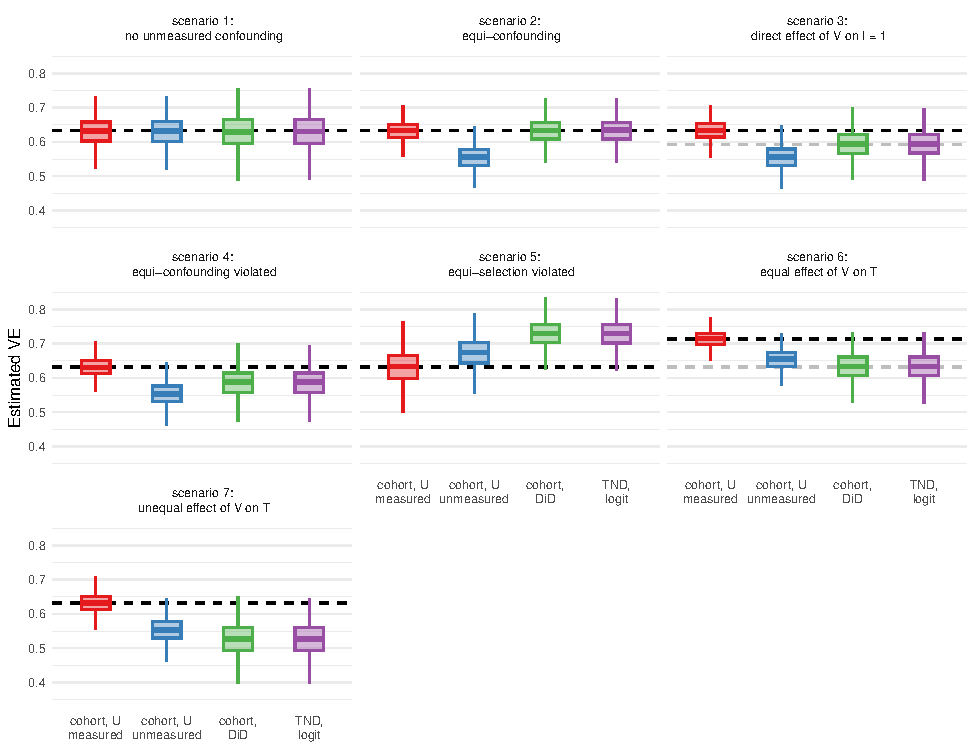
\includegraphics{../results/sims1.pdf}
    \caption{
        Bias of vaccine effectiveness (VE) estimators across different simulation scenarios. In each scenario, we compare: (i) ideal cohort estimator with $U$ measured, (ii) more typical cohort estimator with $U$ unmeasured, (iii) a difference-in-differences (DiD) estimator in the cohort based on equation \ref{eqn:om_estimand}, and (iv) the TND estimator $\widehat{\Psi}_{om}^*$. Results are based on 1000 Monte Carlo replications. Black dashed line is the true VE. In scenario 3, grey dashed line is the ratio of VEs for test-positive versus test-negative illness. In scenarios 6 and 7, grey dashed line VE against symptomatic illness.}
    \label{fig:sims1}
\end{figure}

\begin{figure}
    \centering
    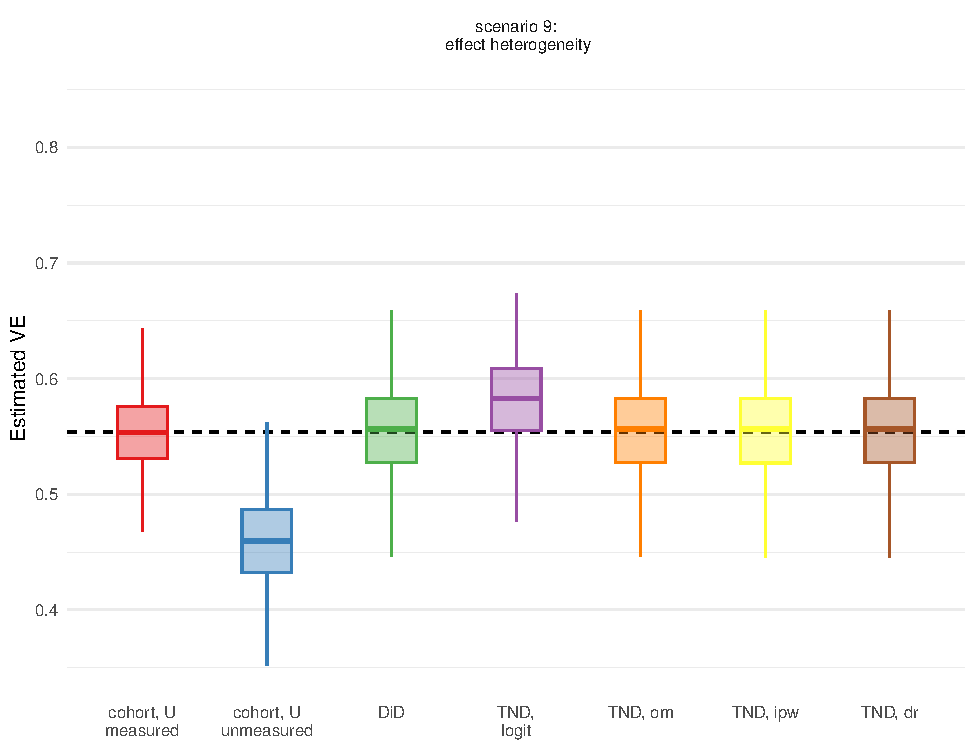
\includegraphics{../results/sims2.pdf}
    \caption{Bias of vaccine effectiveness (VE) estimators under effect heterogeneity. We add to the estimators considered in Figure \ref{fig:sims1} the conventional TND logistic regression estimator (TND, logit) as well as the novel estimators of the marginal RRV introduced in section \ref{sec:estimation}: the outcome modeling estimator (TND, om), the inverse probability weighting estimator (TND, ipw), and the doubly robust estimator (TND, dr). Results are based on 1000 Monte Carlo replications. Black dashed line is the true VE.}
    \label{fig:sims2}
\end{figure}

\clearpage


\begin{appendix}

    \renewcommand{\thefigure}{A\arabic{figure}}
    \setcounter{figure}{0}
    
    \renewcommand{\thetable}{A\arabic{table}}
    \setcounter{table}{0}
    
    \renewcommand{\theequation}{A\arabic{equation}}
    \setcounter{equation}{0}

    \singlespacing
%    \appendixwithtoc
    \newpage

    \section{Proofs of main identifiability results}
    For convenience, we restate the core identifiability assumptions from the main text. 
    \vspace{1em}
    
    \noindent Assumptions:
    \begin{itemize}
        \item[(A1)] Consistency of potential outcomes. For all individuals $i$ and for $v \in \{0, 1\}$, we have $I_i^v = I_i$ and $T_i^v = T_i$ when $V_i = v$.
        \item[(A2)] No effect of vaccination on test-negative symptomatic illness ($I = 1$) among the vaccinated. That is, $\Pr(I^0 = 1 | V = 1, X) = \Pr(I^1 = 1 | V = 1, X).$
        \item[(A3)] Odds ratio equi-confounding. Degree of unmeasured confounding bias on the odds ratio scale is the same for test-positive and test-negative illnesses, i.e. 
        $$\beta_2(X) = \beta_1(X), $$
        $$ \text{where } \beta_i(X) = \log \frac{\Pr(I^0 = i, T^0 = 1 | V = 1, X)\Pr(I^0 = 0, T^0 = 1 | V = 0, X)}{\Pr(I^0 = 0, T^0 = 1 | V = 1, X)\Pr(I^0 = i, T^0 = 1| V = 0, X)}.$$
        \item[(A4)] Overlap of vaccination among test-positives and test-negatives. Define $\mathcal{S}_i(v)$ as the support of the law of $(I^v = i, T^v = 1, V = v, X)$, then for $v$ in $\{0,1\}$, then it must be that $\mathcal{S}_2(1) \subseteq \mathcal{S}_2(0)$ and $\mathcal{S}_2(v) \subseteq \mathcal{S}_1(v).$
        \item[(A5)] No direct effect of vaccination on test-seeking behavior among the vaccinated. That is, for $i$ in $\{1,2\}$, $\Pr[T^1 = 1 | I^1 = i, V = 1, X] = \Pr[T^0 = 1 | I^0 = i, V = 1, X].$
        % \item[(A5)] Equivalent effects of vaccination on test-seeking behavior for test-positive and test-negative illnesses. That is, for $v \in \{0, 1\}$, $\Pr(T^v = 1 | I^v = 2, V = 1, X) = \Pr(T^v = 1 | I^v = 1, V = 1, X)$ and $\Pr(T^v = 1 | I^v = 2, V = 0, X) = \Pr(T^v = 1 | I^v = 1, V = 0, X)$.
    \end{itemize}

    In Proposition \ref{prop1}, we establish that, under consistency alone, the causal risk ratio among the vaccinated, $\Psi_{RRV}$, is equivalent to two expressions involving the (unobserved) treatment-free potential outcome $I^0 = 2$, one based on the outcome itself and one based on the so-called generalized propensity score. In Theorem \ref{theorem1}, we show that, if we add assumptions A2-A4, we can use the observed incidence of the test-negative illness $I = 1$ as a proxy for expressions involved the treatment-free potential outcome, $I^0 = 2$, and therefore identify $\Psi_{RRV}$ if we had access to all symptomatic infections in the underlying cohort. Then in Corollary \ref{corollary1} we show that adding assumption A5 allows us to identify $\Psi_{RRV}$ in the underlying cohort if we only observe infections among those who seek tests. Finally, in Corollary \ref{corollary2} we show $\Psi_{RRV}$ is still identifiable under the sampling design of the TND, due to the invariance of the odds ratio. 
    
    \newpage
    \begin{proposition}\label{prop1}
    Under assumption A1, the causal risk ratio among the vaccinated, 
    \begin{equation*}
        \Psi \equiv \dfrac{\Pr(I^1=2|V=1)}{\Pr(I^0=2|V=1)},
    \end{equation*}
    is equivalent to 
    \begin{equation}
        \Psi^0_{om} \equiv \dfrac{\Pr(I = 2 | V = 1)}{E\left[\Pr(I = 2 | V = 0, X) \exp\{\alpha^0_2(X)\}\Big| V = 1 \right]}
    \end{equation}
    and 
    \begin{equation}
        \Psi^0_{ipw} \equiv \dfrac{E\{V \mathbbm 1(I = 2)\}}{E\left\{ (1 - V) \mathbbm 1(I = 2) \dfrac{\pi^0_2(X)}{1 - \pi^0_2(X)}\right\}}
    \end{equation}
    where 
    \begin{equation*}
        \pi^0_i(X) = \Pr(V = 1 | I^0 = i, X)
    \end{equation*}
    is the generalized propensity score and 
    \begin{equation*}
        \beta^0_i(X) = \log \dfrac{\Pr(I^0 = i | V = 1, X)\Pr(I^0 = 0 | V = 0, X)}{\Pr(I^0 = 0 | V = 1, X)\Pr(I^0 = i | V = 0, X)}
    \end{equation*}
    is the odds ratio comparing the treatment-free potential outcome in the vaccinated and unvaccinated groups with 
    \begin{equation*}
        \eta^0(X) = \log \dfrac{\Pr(I^0 = 0 | V = 0, X)}{\Pr(I^0 = 0 | V = 1, X)}
    \end{equation*}
    and 
    \begin{equation*}
        \alpha^0_i(X) = \log \dfrac{\Pr(I^0 = i | V = 1, X)}{\Pr(I^0 = i | V = 0, X)}
    \end{equation*}
    such that
    \begin{equation*}
        \beta^0_i(X) = \eta^0(X) + \alpha^0_i(X).
    \end{equation*}
    \end{proposition}
    
    \begin{proof}
    For the first expression, we have 
    \begin{align*}
        \Psi &= \dfrac{\Pr(I^1=2|V=1)}{\Pr(I^0=2|V=1)} \\
        &= \dfrac{\Pr(I^1=2|V=1)}{E[E\{\mathbbm 1 (I^0 = 2) | V = 1, X\} | V = 1]} \\
        &= \dfrac{\Pr(I^1=2|V=1)}{E\left\{\int \mathbbm 1 (I^0 = 2) \cdot f(I^0 = i | V = 1, X) di \mid  V = 1\right\}} \\
        &= \dfrac{\Pr(I^1=2|V=1)}{E\left\{\int \mathbbm 1 (I^0 = 2) \cdot f(I^0 = i | V = 0, X) \dfrac{f(I^0 = i | V = 1, X)}{f(I^0 = i | V = 0, X)}di \mid  V = 1\right\}} \\
        &= \dfrac{\Pr(I^1=2|V=1)}{E\left\{ \Pr(I^0 = 2 | V = 0, X) \dfrac{\Pr(I^0 = 2 | V = 1, X)}{\Pr(I^0 = 2 | V = 0, X)} \mid  V = 1\right\}} \\
        &= \dfrac{\Pr(I=2|V=1)}{E\left[ \Pr(I = 2 | V = 0, X) \exp\{\alpha^0_2(X)\} \mid  V = 1\right]}.
    \end{align*}
    The first line restates the definition. The second uses the law of iterated expectation. The third applies the definition of conditional expectation. The fourth multiplies the density by one. The fifth evaluates the integral and the sixth applies consistency and the definition of $\alpha_i(X)$
    
    For the second, we have 
    \begin{align*}
        \Psi &= \dfrac{\Pr(I^1=2|V=1)}{\Pr(I^0=2|V=1)} \\
        &= \dfrac{E\left\{\dfrac{V}{\Pr(V = 1)} \mathbbm 1 (I^1 = 2)\right\}}{E\left\{\dfrac{V}{\Pr(V=1)}\mathbbm 1 (I^0 = 2)\right\}} \\
        &= \dfrac{E\{V \mathbbm 1 (I^1 = 2)\}}{E\left\{\mathbbm 1 (I^0 = 2) E(A | I^0 = 2, X)\right\}} \\
        &= \dfrac{E\{V \mathbbm 1 (I^1 = 2)\}}{E\left\{\mathbbm 1 (I^0 = 2) \pi^0_2(X)\right\}} \\
        &= \dfrac{E\{V \mathbbm 1 (I^1 = 2)\}}{E\left\{\mathbbm 1 (I^0 = 2) \dfrac{\pi^0_2(X)}{1-\pi^0_2(X)}E(1-A|I^0 = 2, X)\right\}} \\
        &= \dfrac{E\{V \mathbbm 1 (I = 2)\}}{E\left\{(1 - V)\mathbbm 1 (I = 2) \dfrac{\pi^0_2(X)}{1-\pi^0_2(X)}\right\}}.
    \end{align*}
    The first line restates the definition. The second uses the definition of conditional expectation. The third applies the law of iterated expectation. The fourth applies the definition of the generalized propensity score $\pi_i(X)$. The fifth multiplies by one. The sixth reverses the law of iterated expectations and applies consistency. 
    \end{proof}
    \newpage
    
    \begin{theorem}\label{theorem1}
    Under assumptions A1 - A4, the causal risk ratio among the vaccinated, 
    \begin{equation*}
        \Psi \equiv \dfrac{\Pr(I^1=2|V=1)}{\Pr(I^0=2|V=1)},
    \end{equation*}
    is identified in the population underlying the test-negative design by 
    \begin{equation}
        \Psi_{om} \equiv \dfrac{\Pr(I = 2 | V = 1)}{E\left\{ \exp\{\alpha_1(X)\} \Pr(I = 2 | V = 0, X) \Big| V = 1 \right\}}
    \end{equation}
    and 
    \begin{equation}
        \Psi_{ipw} \equiv \dfrac{E\{V \mathbbm 1 (I = 2)\}}{E\left\{ (1 - V) \mathbbm 1(I = 2) \dfrac{\pi_1(X)}{1 - \pi_1(X)}\right\}}
    \end{equation}
    where $\alpha_i(X) = \log \dfrac{\Pr(I =i | V = 1, X)}{\Pr(I =i | V = 0, X)}$ and $\pi_i(X) = \Pr(V = 1 | I = i, X)$ are both observables. 
    \end{theorem}
    
    \begin{proof}
    For the first expression, note that by Assumption A3 and exclusivity of test-negative and test-positive illnesses
    \begin{align*}
        \dfrac{\Pr(I^0 = 2 | V = 1, X)}{\Pr(I^0 = 2 | V = 0, X)} &= \dfrac{\Pr(I^0 = 1 | V = 1, X)}{\Pr(I^0 = 1 | V = 0, X)} \\
        &= \dfrac{\Pr(I^1 = 1 | V = 1, X)}{\Pr(I^0 = 1 | V = 0, X)} \\
        &= \dfrac{\Pr(I = 1 | V = 1, X)}{\Pr(I = 1 | V = 0, X)} \\
    \end{align*}
    where the first line is by Assumption A3 and exclusivity of test-negative and test-positive illnesses. The second line is by Assumption A2. And the last line applies consistency. This implies
    \begin{equation*}
        \alpha_2^0(X) = \alpha_1(X)
    \end{equation*}
    and, therefore, combining with the derivation of Proposition \ref{prop1}, we have
    \begin{align*}
        \Psi &= \dfrac{\Pr(I = 2 | V = 1)}{E\left\{ \exp\{\alpha^0_2(X)\} \Pr(I = 2 | V = 0, X) \Big| V = 1 \right\}} \\
        &= \dfrac{\Pr(I = 2 | V = 1)}{E\left\{ \exp\{\alpha_1(X)\} \Pr(I = 2 | V = 0, X) \Big| V = 1 \right\}}.
    \end{align*}
    
    For the second expression, note first that, by the invariance of odds ratios, Assumptions A2 and A3 imply
    \begin{equation*}
        \dfrac{\Pr(V = 1 | I^0 = 2, X)}{\Pr(V = 0 | I^0 = 2, X)} = \dfrac{\Pr(V = 1 | I = 1, X)}{\Pr(V = 0 | I = 1, X)}
    \end{equation*}
    and by consequence 
    \begin{equation*}
        \dfrac{\pi^0_2(X)}{1 - \pi^0_2(X)} = \dfrac{\pi_1(X)}{1 - \pi_1(X)}.
    \end{equation*}
    Thus, again, continuing the derivation in Theorem 1, we have 
    \begin{align*}
        \Psi &= \dfrac{E\{V \mathbbm 1 (I = 2)\}}{E\left\{(1 - V)\mathbbm 1 (I = 2) \dfrac{\pi^0_2(X)}{1-\pi^0_2(X)}\right\}} \\
        &= \dfrac{E\{V \mathbbm 1 (I = 2)\}}{E\left\{(1 - V)\mathbbm 1 (I = 2) \dfrac{\pi_1(X)}{1-\pi_1(X)}\right\}}.
    \end{align*}
    \end{proof}
    \newpage
    
    \begin{corollary}\label{corollary1}
    If we add assumption A5, that is that direct effects of vaccination on testing behavior are the same for test-positive and test-negative illnesses, then $\Psi_{om}$ and $\Psi_{ipw}$ are equivalent to
    \begin{equation}
        \Psi^\dagger_{om} \equiv \dfrac{\Pr(I = 2, T = 1 | V = 1)}{E\left\{ \exp\{\alpha^\dagger_1(X)\} \Pr(I = 2, T = 1 | V = 0, X) \Big| V = 1 \right\}}
    \end{equation}
    and 
    \begin{equation}
        \Psi^\dagger_{ipw} \equiv \dfrac{E\{V \mathbbm 1 (I = 2, T = 1)\}}{E\left\{ (1 - V) \mathbbm 1(I = 2, T = 1) \dfrac{\pi^\dagger_1(X)}{1 - \pi^\dagger_1(X)}\right\}}
    \end{equation}
    where $\alpha^\dagger_1(X) = \dfrac{\Pr(I = 1, T = 1 | V = 1, X)}{\Pr(I = 1, T = 1 | V = 0, X)}$ and $\pi^\dagger_1(X) = \Pr(V = 1| I = 1, T = 1, X)$.
    \end{corollary}
    
    \begin{proof}
        Define $\Psi^\dagger$ as 
        \begin{equation*}
            \Psi^\dagger \equiv  \dfrac{\Pr(I^1=2, T^1 = 1|V=1)}{\Pr(I^0=2, T^0 = 1|V=1)},
        \end{equation*}
        and note that
        \begin{align*}
            \Psi^\dagger &= \dfrac{\Pr(I^1=2, T^1 = 1|V=1)}{\Pr(I^0=2, T^0 = 1|V=1)} \\
            &= \dfrac{\Pr(I^1 = 2 | V = 1)\Pr(T^1 = 1 | I^1 = 2, V = 1)}{\Pr(I^0=2|V=1)\Pr(T^0 = 1 | I^0 = 2, V = 1)} \\
            & = \dfrac{\Pr(I^1 = 2 | V = 1)}{\Pr(I^0 = 2 | V = 1)} \\
            &= \Psi.
        \end{align*}
        The first line follows by definition, the second factors the joint probability, and the third applies applies assumption A3. 
    
        As $\Psi^\dagger = \Psi$, it now suffices to show that $\Psi^\dagger_{om}$ and $\Psi^\dagger_{ipw}$ identify $\Psi^\dagger$. Following the same steps as the derivations in Theorems 1 and 2, for the first expression we have 
        \begin{align*}
        \Psi^\dagger &= \dfrac{\Pr(I^1=2, T^1 = 1|V=1)}{\Pr(I^0=2, T^0 = 1|V=1)} \\
        &= \dfrac{\Pr(I^1=2, T^1 = 1|V=1)}{E[E\{\mathbbm 1 (I^0 = 2, T^0 = 1) | V = 1, X\} | V = 1]} \\
        &= \dfrac{\Pr(I^1=2, T^1 = 1|V=1)}{E\left\{\int \mathbbm 1 (I^0= 2, T^0 = 1) \cdot f(I^0 = i, T^0 = 1 | V = 1, X) di \mid  V = 1\right\}} \\
        &= \dfrac{\Pr(I^1=2, T^1 = 1|V=1)}{E\left\{\int \mathbbm 1 (I^0= 2, T^0 = 1) \cdot f(I^0 = i, T^0 = 1 | V = 0, X) \dfrac{f(I^0 = i, T^0 = 1 | V = 1, X)}{f(I^0 = i, T^0 = 1 | V = 0, X)}di \mid  V = 1\right\}} \\
        &= \dfrac{\Pr(I^1=2, T^1 = 1|V=1)}{E\left\{ \Pr(I^0 = 2, T^0 = 1 | V = 0, X) \dfrac{\Pr(I^0 = 2, T^0 = 1 | V = 1, X)}{\Pr(I^0 = 2, T^0 = 1 | V = 0, X)} \mid  V = 1\right\}} \\
        &= \dfrac{\Pr(I^1=2, T^1 = 1|V=1)}{E\left\{ \Pr(I^0 = 2, T^0 = 1 | V = 0, X) \dfrac{\Pr(I^0 = 1, T^0 = 1 | V = 1, X)}{\Pr(I^0 = 1, T^0 = 1 | V = 0, X)} \mid  V = 1\right\}} \\
        &= \dfrac{\Pr(I^1=2, T^1 = 1|V=1)}{E\left\{ \Pr(I^0 = 2, T^0 = 1 | V = 0, X) \dfrac{\Pr(I^1 = 1, T^1 = 1 | V = 1, X)}{\Pr(I^0 = 1, T^0 = 1 | V = 0, X)} \mid  V = 1\right\}} \\
        &= \dfrac{\Pr(I=2, T = 1|V=1)}{E\left\{ \Pr(I = 2, T = 1 | V = 0, X) \dfrac{\Pr(I = 1, T = 1 | V = 1, X)}{\Pr(I = 1, T = 1 | V = 0, X)} \mid  V = 1\right\}} \\
        &= \dfrac{\Pr(I = 2, T = 1 | V = 1)}{E\left\{ \exp\{\alpha^\dagger_1(X)\} \Pr(I = 2, T = 1 | V = 0, X) \Big| V = 1 \right\}}.
        \end{align*}
    
    For the second expression, note first that, by the invariance of odds ratios, Assumptions A2, A3, and A5 imply
    \begin{equation*}
        \dfrac{\Pr(V = 1 | I^0 = 2, T^0 = 1, X)}{\Pr(V = 0 | I^0 = 2,  T^0 = 1, X)} = \dfrac{\Pr(V = 1 | I = 1, T = 1, X)}{\Pr(V = 0 | I = 1,  T = 1, X)}
    \end{equation*}
    and by consequence 
    \begin{equation*}
        \dfrac{\pi^{0\dagger}_2(X)}{1 - \pi^{0\dagger}_2(X)} = \dfrac{\pi^\dagger_1(X)}{1 - \pi^\dagger_1(X)}.
    \end{equation*}
    Thus we have
    \begin{align*}
        \Psi &= \dfrac{\Pr(I^1=2, T^1 = 1|V=1)}{\Pr(I^0=2, T^0 = 1|V=1)} \\
        &= \dfrac{E\{\dfrac{V}{\Pr(V=1)} \mathbbm 1 (I^1 = 2, T^1 = 1)\}}{E\left\{\dfrac{V}{\Pr(V=1)}\mathbbm 1 (I^0 = 2, T^0 = 1)\right\}} \\
        &= \dfrac{E\{V \mathbbm 1 (I^1 = 2, T^1 = 1)\}}{E\left\{\mathbbm 1 (I^0 = 2, T^0 = 1) E(A | I^0 = 2, T^0 = 1, X)\right\}} \\
        &= \dfrac{E\{V \mathbbm 1 (I^1 = 2, T^1 = 1)\}}{E\left\{\mathbbm 1 (I^0 = 2, T^0 = 1) \pi^{0\dagger}_2(X)\right\}} \\
        &= \dfrac{E\{V \mathbbm 1 (I^1 = 2, T^1 = 1)\}}{E\left\{\mathbbm 1 (I^0 = 2, T^0 = 1) \dfrac{\pi^{0\dagger}_2(X)}{1-\pi^{0\dagger}_2(X)}E(1-A|I^0 = 2, T^0 = 1, X)\right\}} \\
        &= \dfrac{E\{V \mathbbm 1 (I = 2, T = 1)\}}{E\left\{(1 - V)\mathbbm 1 (I = 2, T = 1) \dfrac{\pi^{0\dagger}_2(X)}{1-\pi^{0\dagger}_2(X)}\right\}} \\
        &= \dfrac{E\{V \mathbbm 1 (I = 2, T = 1)\}}{E\left\{(1 - V)\mathbbm 1 (I = 2, T = 1) \dfrac{\pi^\dagger_1(X)}{1-\pi^\dagger_1(X)}\right\}}.
    \end{align*}
    \end{proof}
    \newpage 
    \begin{corollary}\label{corollary2}
    Under assumptions A1 - A5 and the biased sampling design of the test-negative study, $\Psi^\dagger_{om}$ and $\Psi^\dagger_{ipw}$, and therefore by previous results $\Psi_{om}$, $\Psi_{ipw}$, and $\Psi$, are identified by
    \begin{equation}
        \Psi_{om}^* = \dfrac{\Pr(I^* = 1 | S = 1, V = 1)}{E\left\{ \exp\{\alpha^*_1(X)\} \Pr(I^* = 1 | S = 1, V = 0, X) \Big| S = 1, V = 1 \right\}}
    \end{equation}
    and 
    \begin{equation}
        \Psi_{ipw}^* = \dfrac{E\{VI^*|S =1\}}{E\left\{ (1 - V) I^* \dfrac{\pi^*(X)}{1 - \pi^*(X)} \bigg| S = 1\right\}}
    \end{equation}
    where $\alpha^*_1(X) = \dfrac{\Pr(I^* = 0 | S = 1, V = 1, X)}{\Pr(I^* = 0| S = 1, V = 0, X)}$ and $\pi^*(X) = \Pr(V = 1| S = 1, I^* = 0, X)$.
    \end{corollary}
    
    \begin{proof}
    For the first expression we have,
        \begin{align*}
        \Psi^\dagger_{om} &= \dfrac{\Pr(I=2, T = 1|V=1)}{E\left\{ \dfrac{\Pr(I = 1, T = 1 | V = 1, X)}{\Pr(I = 1, T = 1 | V = 0, X)}\Pr(I = 2, T = 1 | V = 0, X) \mid  V = 1\right\}} \\
        &= \dfrac{\Pr(I = 2, T = 1 | V = 1)}{\int \dfrac{\Pr(I = 1, T = 1 | V = 1, x)}{\Pr(I = 1, T = 1 | V = 0, x)} \Pr(I = 2, T = 1 | V = 0, x) f(x | V = 1) dx} \\
        &= \dfrac{\Pr(I = 2 | T = 1, V = 1)\Pr(T = 1 | V = 1)}{\int \dfrac{\Pr(I = 1 | T = 1, V = 1, x)}{\Pr(I = 1 | T = 1, V = 0, x)} \Pr(I = 2 | T = 1, V = 0, x) \Pr(T = 1 | V = 1, x) f(x | V = 1) dx} \\
        &= \dfrac{\Pr(I = 2 | T = 1, V = 1)\Pr(T = 1 | V = 1)}{\int \dfrac{\Pr(I = 1 | T = 1, V = 1, x)}{\Pr(I = 1 | T = 1, V = 0, x)} \Pr(I = 2 | T = 1, V = 0, x) \Pr(T = 1 | V = 1) f(x | T =1, V = 1) dx} \\
        &= \dfrac{\Pr(I = 2 | T = 1, V = 1)}{\int \dfrac{\Pr(I = 1 | T = 1, V = 1, x)}{\Pr(I = 1 | T = 1, V = 0, x)} \Pr(I = 2 | T = 1, V = 0, x) f(x | T =1, V = 1) dx} \\
        &= \dfrac{\Pr(I = 2 | T = 1, V = 1)}{E\left\{ \dfrac{\Pr(I = 1 | T = 1, V = 1, X)}{\Pr(I = 1 | T = 1, V = 0, X)} \Pr(I = 2 | T = 1, V = 0, X) \bigg| T = 1, V = 1\right\}} \\
        &= \dfrac{\Pr(I^* = 1 | S = 1, V = 1)}{E\left\{ \dfrac{\Pr(I^* = 0 | S = 1, V = 1, X)}{\Pr(I^* = 0 | S = 1, V = 0, X)} \Pr(I^* = 1 | S = 1, V = 0, X) \bigg| S = 1, V = 1\right\}} \\
        &= \dfrac{\Pr(I^* = 1 | S = 1, V = 1)}{E\left\{ \exp\{\alpha^*_1(X)\} \Pr(I^* = 1 | S = 1, V = 0, X) \Big| S = 1, V = 1 \right\}}.
    \end{align*}
    The first line restates the definition of $\Psi^\dagger_{om}$. The second applies the definition of conditional expectation. The third factors the joint probabilities. The fourth applies Bayes theorem, i.e. 
    \begin{equation*}
        f(x | V = 1) = \dfrac{f(x | T = 1, V = 1)\Pr(T = 1 | V = 1)}{\Pr(T = 1 | V = 1, x)}.
    \end{equation*}
    The fifth cancels the $\Pr(T = 1 |V = 1)$ terms in the numerator and denominator. The sixth applies the definition of conditional expectation. The seventh applies the sampling design $S = \mathbbm 1 (T = 1, I \neq 0)$ and the perfect test $I^* = \mathbbm 1(I = 2)$.
    
    For the second expression we have,
    \begin{align*}
        \Psi^\dagger_{ipw} &= \dfrac{E\{V \mathbbm 1 (I = 2, T = 1)\}}{E\left\{ (1 - V) \mathbbm 1(I = 2, T = 1) \dfrac{\pi^\dagger_1(X)}{1 - \pi^\dagger_1(X)}\right\}} \\
        &= \dfrac{E\{V \mathbbm 1 (I = 2) | T = 1\} \Pr(T = 1)}{E\left\{ (1 - V) \mathbbm 1(I = 2) \dfrac{\pi^\dagger_1(X)}{1 - \pi^\dagger_1(X)} \bigg| T = 1\right\} \Pr(T = 1)} \\
        &= \dfrac{E\{V \mathbbm 1 (I = 2) | T = 1\}}{E\left\{ (1 - V) \mathbbm 1(I = 2) \dfrac{\pi^\dagger_1(X)}{1 - \pi^\dagger_1(X)} \bigg| T = 1\right\}} \\
        &= \dfrac{E\{VI^*|S =1\}}{E\left\{ (1 - V) I^* \dfrac{\pi^*(X)}{1 - \pi^*(X)} \bigg| S = 1\right\}}.
    \end{align*}
    The first line restates the definition of $\Psi^\dagger_{ipw}$. The second applies the law of iterated expectations. The third cancels the $\Pr(T = 1)$ terms in the numerator and denominator. The fourth applies the sampling design $S = \mathbbm 1 (T = 1, I \neq 0)$ and the perfect test $I^* = \mathbbm 1(I = 2)$.
    
    \end{proof}
    \newpage
    \section{Estimation}
    \subsection{Plug-in}
    Corollary \ref{corollary2} suggests two plug-in estimators for the causal risk ratio among the vaccinated.  An estimator based on modeling the outcome
    \begin{equation}
        \widehat{\Psi}_{om}^* = \dfrac{\sum_{i=1}^n V_i I^*_i}{\sum_{i=1}^n V_i \mu_0(X_i)\dfrac{1 - \mu^*_1(X_i)}{1 - \mu^*_0(X_i)}},
    \end{equation}
    and an inverse probability weighting estimator
    \begin{equation}
        \widehat{\Psi}_{ipw}^* = \dfrac{\sum_{i=1}^n V_i I^*_i}{\sum_{i=1}^n (1 - V_i) I^*_i \dfrac{\pi^*(X_i)}{1 - \pi^*(X_i)}},
    \end{equation}
    where 
    \begin{align*}
        \pi^*(X) &= \Pr(V=1\mid S=1, I^*=0, X) \\
        \mu^*_v(X) &= \Pr(I^*=1\mid S=1, V=v, X).
    \end{align*}

\subsection{Doubly robust}
We consider a 
\begin{equation}\label{eqn:dr_estimator}
\widehat{\Psi}_{dr}^* = \dfrac{\sum_{i=1}^n V_i I^*_i}{\sum_{i=1}^n (1 - V_i)\dfrac{\pi^*_1(X_i)}{1 - \pi^*_1(X_i)} \{I_i - \mu^*_0(X_i) \} + V_i \mu^*_0(X_i)\dfrac{1 - \mu^*_1(X_i)}{1 - \mu^*_0(X_i)}}
\end{equation}

To prove the doubly-robustness of $\widehat{\Psi}^*_{dr}$, it suffices to show that 
\begin{align*}
    E\bigg[ (1 - V)\dfrac{\pi^*_1(X)}{1 - \pi^*_1(X)} \{I - \mu^*_0(X) \} + V \mu^*_0(X)\dfrac{1 - \mu^*_1(X)}{1 - \mu^*_0(X)}\mid S=1\bigg] = \Pi
\end{align*}
if (1) $\dot\mu^*_v(\cdot)=\mu^*_v(\cdot)$ a.s. for $v=0,1$, or (2) $\dot \pi^*(\cdot)=\pi^*(\cdot)$ and $\dot\mu_0(\cdot)=\mu_0(\cdot)$  a.s.

    \begin{enumerate}
        \item If $\dot\mu_v(\cdot)=\mu_v(\cdot)$ a.s. for $v=0,1$, then
        \begin{align*}
            &E\bigg[ (1-V)\{I^* -  \mu_0(X)\}\dfrac{\dot\pi(X)\{1 - \mu_1(X)\}}{\{1 - \dot\pi(X)\}\{1 - \mu_0(X)\}^2} + V\{1-I^*\}\dfrac{\mu_0(X)}{1-\mu_0(X)}\mid S=1\bigg]\\
            =& E\bigg[ \{I^* -  \mu_0(X)\}\dfrac{\dot\pi(X)\{1 - \mu_1(X)\}}{\{1 - \dot\pi(X)\}\{1 - \mu_0(X)\}^2} \mid V=0, S=1\bigg]Pr(V=0\mid  S=1) + \\
            &\qquad E\bigg[E\{V(1-I^*)\mid X\}\dfrac{\mu_0(X)}{1-\mu_0(X)}\mid  S=1\bigg]\\
            =& E\bigg[E \{I^* -  \mu_0(X)\mid V=0, S=1, X\}\dfrac{\dot\pi(X)\{1 - \mu_1(X)\}}{\{1 - \dot\pi(X)\}\{1 - \mu_0(X)\}^2} \mid V=0, S=1\bigg]Pr(V=0\mid  S=1) + \\
            &\qquad E\bigg[\pi(X)\{1-\mu_1(X)\}\dfrac{\mu_0(X)}{1-\mu_0(X)}\mid  S=1\bigg]\\
            &= 0 + \Pi = \Pi
        \end{align*}
    \item If $\dot\pi(\cdot)=\pi(\cdot)$ and $\dot\mu_0(\cdot)=\mu_0(\cdot)$ a.s., then 
\begin{align*}
    &E\bigg[ (1-V)\{I^* -  \mu_0(X)\}\dfrac{\pi(X)\{1 - \dot\mu_1(X)\}}{\{1 - \pi(X)\}\{1 - \mu_0(X)\}^2} + V\{1-I^*\}\dfrac{\mu_0(X)}{1-\mu_0(X)}\mid S=1\bigg]\\
    =& E\bigg[ \{1 - \pi(X)\}\{\mu_0(X) -  \mu_0(X)\}\dfrac{\pi(X)\{1 - \dot\mu_1(X)\}}{\{1 - \pi(X)\}\{1 - \mu_0(X)\}^2} + \pi(X)\{1-\mu_1(X)\}\dfrac{\mu_0(X)}{1-\mu_0(X)}\mid S=1\bigg]\\
    &= \Pi
\end{align*}


    \end{enumerate}
    \subsection{Efficient influence function}
    Let $\Psi(P)$ be the target parameter under true law of the observed data $P$. From the identifiability results in Section 1, we have that 
% $$\Psi(P) = \dfrac{E(I^*\mid S=1, V=1)}{E\left\{\dfrac{\Pr(I^*=1\mid S=1, V=0, X)\Pr(V=1\mid S=1, I^*=0, X)}{\Pr(V=0\mid S=1, I^*=0, X)}\mid S=1, V=1\right\}}.$$ 
$$\Psi(P) = E\left\{\dfrac{\Pr(I^*=1\mid S=1, V=0, X)\Pr(I^*=0\mid S=1, V=1, X)}{\Pr(I^*=0\mid S=1, V=0, X)}\mid S=1, V=1\right\}.$$ 
For convenience, let
\begin{align*}
    \pi(X) &= \Pr(V=1\mid S=1, I^*=0, X) \\
    \mu^*_v(X) &= \Pr(I^*=1\mid S=1, V=v, X).
\end{align*}
Define $P_t$ as a parametric submodel indexed by $t \in [0,1]$ such that
$$P_t = t \widetilde{P} + (1 - t)P$$
where $\widetilde{P}$ is smoothed parametric estimate of $P$ and note that $P_0 = P$. To find the influence function we will use the fact that if we perturb the target in direction of a point mass $\widetilde{o} = (\widetilde{i}^*, \widetilde{s}, \widetilde{v}, \widetilde{x})$ of $\widetilde{P}$
$$ \chi(P, \widetilde{o}) = \frac{d}{dt} \Psi(P_t)\bigg\vert_{t=0}$$
where the right-hand side is the so-called the G\^{a}teaux derivative. Note that 
\begin{align*}
    \Psi(P_t) &= \int \dfrac{\int i^* f_t(i^* | s=1,v=0,x)di^* \int (1-i^*) f_t(i^* | s=1, v=1, x)di^*}{\int(1 - i^*) f_t(i^* | s=1, v=0, x)di^*}f_t(x|s=1,v=1)dx \\
    &= \int \dfrac{1}{f_{S,V}(1, 1)} \dfrac{\int i^* f_t(i^*, s=1,v=0,x)di^* \int (1 - i^*)  f_t(i^*, s=1, v=1, x)dv}{\int(1 - i^*)  f_t(i^*, s=1, v=0, x)dv}dx 
\end{align*}
\begin{align*}
    \Psi(P_t) &= \int (1 - v)i^*\dfrac{\int v f_t(v | s=1, i^*=0, x)dv}{\int (1-v) f_t(v | s=1, i^*=0, x)dv} f(i^*, s=1, v, x) di^* dv dx \\
    &= \int (1 - v)i^*\dfrac{\int v f_t(v, s=1, i^*=0, x)dv}{\int (1-v) f_t(v, s=1, i^*=0, x)dv} f(i^*, s=1, v, x) di^* dv dx
\end{align*}

Then the pathwise derivative of $\Psi_t$ wrt $t$ is
\begin{align*}
   &\frac{d}{dt} \Psi(P_t)\bigg\vert_{t=0} \\
   &= \int \dfrac{1}{f_{S,V}(1, 1)} \frac{d}{dt} \left\{\dfrac{\int i^* f_t(i^*, s=1,v=0,x)di^* \int (1 - i^*)  f_t(i^*, s=1, v=1, x)dv}{\int(1 - i^*)  f_t(i^*, s=1, v=0, x)dv} \right\} \bigg\vert_{t=0}dx \\
   &= \int \dfrac{1}{f_{S,V}(1, 1)}\bigg\{ \dfrac{1 - \mu^*_1(x)}{1-\mu^*_0(x)} \dfrac{f(x, s=1, v=1)}{f(x, s=1, v=0)}\int i^* \frac{d}{dt} f_t(i^*, s=1,v=0,x) \bigg\vert_{t=0} di^* \\
   &\qquad + \dfrac{\mu^*_0(x)}{1 - \mu^*_0(x)} \int (1-i^*) \frac{d}{dt}f_t(i^*, s=1, v=1, x) \bigg\vert_{t=0} di^* \\ 
   &\qquad - \dfrac{\mu^*_0(x)\{1 - \mu^*_1(x)\}}{\{1 - \mu^*_0(x)\}^2} \dfrac{f(x, s=1, v=1)}{f(x, s=1, v =0)} \int (1-i^*) \frac{d}{dt}f_t(i^*, s=1, v=0, x) \bigg\vert_{t=0} dv \\
   % &\qquad + \dfrac{\mu^*_0(x)\pi(x)}{1-\pi(x)} \frac{d}{dt} f_t(x, s=1, v=1) \bigg\vert_{t=0} \\
   % &\qquad - \dfrac{\mu^*_0(x)\pi(x)}{1-\pi(x)} \dfrac{f(x, s=1, v=1)}{f(x, s=1, v=0)} \frac{d}{dt} f_t(x, s=1, v=0) \bigg\vert_{t=0} \bigg\}dx \\
   &= \int \dfrac{1}{f_{S,V}(1, 1)}\bigg\{  \dfrac{1 - \mu^*_1(x)}{1-\mu^*_0(x)} \dfrac{f(x, s=1, v=1)}{f(x, s=1, v=0)}\int i^* \{ \mathbbm 1_{\widetilde i^*, \widetilde s, \widetilde v, \widetilde x}(i^*, 1, 0, x) - f(i^*, s=1,v=0,x) \} di^* \\
   &\qquad + \dfrac{\mu^*_0(x)}{1-\mu^*_0(x)} \int (1 - i^*) \{\mathbbm 1_{\widetilde i^*, \widetilde s, \widetilde v, \widetilde x}(i^*, 1, 1, x) - f(i^*, s=1, v=1, x) \} di^* \\ 
   &\qquad -\dfrac{\mu^*_0(x)\{1 - \mu^*_1(x)\}}{\{1 - \mu^*_0(x)\}^2} \dfrac{f(x, s=1, v=1)}{f(x, s=1, v =0)} \int (1 - i^*) \{\mathbbm 1_{\widetilde i^*, \widetilde s, \widetilde v, \widetilde x}(i^*, 1, 0, x) - f(i^*, s=1, v=0, x) \} di^*  \\
   % & \qquad + \dfrac{\mu^*_0(x)\pi(x)}{1-\pi(x)} \left\{\mathbbm 1_{\widetilde s, \widetilde v, \widetilde x}(1,1,x) - f_t(x, s=1, v=1) \right\} \\
   % & \qquad - \dfrac{\mu^*_0(x)\pi(x)}{1-\pi(x)} \dfrac{f(x, s=1, v=1)}{f(x, s=1, v=0)} \left\{\mathbbm 1_{\widetilde s, \widetilde v, \widetilde x}(1,0,x) - f_t(x, s=1, v=0) \right\}  \bigg\}dx\\
    %&= \int \dfrac{1}{f_{S,V}(1, 1)}\bigg\{ \dfrac{\pi(\widetilde x)}{1-\pi(\widetilde x)} \widetilde i^* \widetilde s(1 - \widetilde v) - \Psi(P) + \dfrac{\mu^*_0(\widetilde x)}{1-\pi(\widetilde x)}(1-\widetilde i^*) \widetilde s \widetilde v  - \Psi(P) - \dfrac{\mu^*_0(x)\pi(x)}{\{1 - \pi(x)\}^2} (1-\widetilde i^*) \widetilde s (1-\widetilde v) - \Psi(P) +  \bigg\}dx \\ 
   &= \int \dfrac{1}{f_{S,V}(1, 1)} \dfrac{\mu^*_0(x)\{1 - \mu^*_1(x)\}}{1 - \mu^*_0(x)}f(x, s=1, v=1) \bigg\{\dfrac{\widetilde{i}^*\widetilde{s}(1-\widetilde{v})\mathbbm 1_{\widetilde{x}}(x)}{\mu^*_0(x)} + \dfrac{(1-\widetilde{i}^*)\widetilde{s}\widetilde{v}\mathbbm 1_{\widetilde{x}}(x)}{1 - \mu^*_1(x)} \\
   &\qquad - \dfrac{(1-\widetilde{i}^*)\widetilde{s}(1-\widetilde{v})\mathbbm 1_{\widetilde{x}}(x)}{\{1 - \mu^*_0(x)\}}\bigg\} dx - \Psi(P) \\
   &=\dfrac{\widetilde s}{f_{S,V}(1, 1)}  \bigg\{(1 - \widetilde v)\widetilde i^*\dfrac{1 - \mu^*_1(\widetilde x)}{1 - \mu^*_0(\widetilde x)} + \widetilde v (1 - \widetilde i^*) \dfrac{\mu^*_0(\widetilde x)}{1 - \mu^*_0(\widetilde x)} -  (1 - \widetilde v) (1 - \widetilde i^*)\dfrac{\mu^*_0(\widetilde x)\{1 - \mu^*_1(\widetilde x)\}}{\{1 - \mu^*_0(\widetilde x)\}^2}  \bigg\}  - \Psi(P) \\
   &=\dfrac{\widetilde s}{f_{S,V}(1, 1)}  \bigg\{(1 - \widetilde v)\widetilde i^*\dfrac{1 - \mu^*_1(\widetilde x)}{1 - \mu^*_0(\widetilde x)} + \widetilde v \left\{\dfrac{\mu^*_0(\widetilde x)}{1 - \mu^*_0(\widetilde x)} - \widetilde i^* \dfrac{\mu^*_0(\widetilde x)}{1 - \mu^*_0(\widetilde x)}\right\} \\
   &\qquad -  (1 - \widetilde v) \left[\dfrac{\mu^*_0(\widetilde x)\{1 - \mu^*_1(\widetilde x)\}}{\{1 - \mu^*_0(\widetilde x)\}^2} - \widetilde i^*\dfrac{\mu^*_0(\widetilde x)\{1 - \mu^*_1(\widetilde x)\}}{\{1 - \mu^*_0(\widetilde x)\}^2}\right]  \bigg\}  - \Psi(P) \\
   &=\dfrac{\widetilde s}{f_{S,V}(1, 1)}  \bigg\{(1 - \widetilde v) \left[\widetilde i^* - \dfrac{\mu^*_0(\widetilde x)}{1 - \mu^*_0(\widetilde x)}  + \widetilde i^*\dfrac{\mu^*_0(\widetilde x)}{1 - \mu^*_0(\widetilde x)}\right]\dfrac{1 - \mu^*_1(\widetilde x)}{1 - \mu^*_0(\widetilde x)}\\
   &\qquad   + \widetilde v \left[\dfrac{\mu^*_0(\widetilde x)}{1 - \mu^*_0(\widetilde x)} - \widetilde i^* \dfrac{\mu^*_0(\widetilde x)}{1 - \mu^*_0(\widetilde x)}\right] \bigg\}  - \Psi(P) \\
   &=\dfrac{\widetilde s}{f_{S,V}(1, 1)}  \bigg\{(1 - \widetilde v) \left[ \dfrac{\widetilde i^* - \widetilde i^* \mu^*_0(\widetilde x) - \mu^*_0(\widetilde x) + \widetilde i^* \mu^*_0(\widetilde x)}{1 - \mu^*_0(\widetilde x)}\right]\dfrac{1 - \mu^*_1(\widetilde x)}{1 - \mu^*_0(\widetilde x)} \\
   &\qquad + \widetilde v \left[\dfrac{\mu^*_0(\widetilde x)}{1 - \mu^*_0(\widetilde x)} - \widetilde i^* \dfrac{\mu^*_0(\widetilde x)}{1 - \mu^*_0(\widetilde x)}\right]   \bigg\}  - \Psi(P) \\
   &=\dfrac{\widetilde s}{f_{S,V}(1, 1)}  \bigg\{(1 - \widetilde v) \{\widetilde i^* - \mu^*_0(\widetilde x)\}\dfrac{1 - \mu^*_1(\widetilde x)}{1 - \mu^*_0(\widetilde x)} + \widetilde v \mu^*_0(\widetilde x) \dfrac{1 - \mu^*_1(\widetilde x)}{1 - \mu^*_0(\widetilde x)}  \bigg\}  - \Psi(P) 
\end{align*}
    \newpage
    
    \section{Example data generation mechanisms satisfying equi-confounding}

    \newpage
    
    \section{Additional results}
    \subsection{Example mechanisms where key assumptions are violated}
    
    \begin{figure}[p]
    \centering
    \begin{subfigure}{0.8\linewidth}
        \centering
        \begin{tikzpicture}[> = stealth, shorten > = 1pt, auto, node distance = 2cm, inner sep = 0pt,minimum size = 0.5pt, semithick]
            \tikzstyle{every state}=[
              draw = none,
              fill = none
            ]
            \node[state] (x) {$X$};
            \node[state] (v) [right of=x] {$V$};
            \node[state] (i) [right of=v] {$I_2$};
            \node[state] (t) [right of=i] {$T$};
            \node[state] (is) [right of=t] {$I^*$};
            \node[state] (i1) [below of=i] {$I_1$};
            \node[state] (u) [below of=x] {$U$};
            \node[state] (v1) [below of=v] {$V_1$};
   
            \path[->] (x) edge node {} (v);
            \path[->] (x) edge [out=45, in=135] node {} (i);
    
            \path[->] (v) edge node {} (i);
            
            \path[->] (i) edge node {} (t);
            \path[->] (i1) edge node {} (t);
            \path[->] (i1) edge node {} (is);

            \path[->] (x) edge [out=45, in=135] node {} (t);
    
            \path[->] (t) edge node {} (is);
            \path[->] (v1) edge node {} (i1);

            \path[->] (i) edge [out=45, in=135] node {} (is);
            \path[->] (i1) edge [dashed] node {} (i);

    
            \path[->] (u) edge node {} (v1);
            \path[->] (u) edge node {} (v);
            % \path[->] (u) edge [line width=2pt] node {} (i);
            % \path[->] (u) edge [line width=2pt] node {} (t);
            % \path[->] (u) edge [line width=2pt] node {} (i1);
            \end{tikzpicture}
        \caption{Correlated vaccination behavior.}
        \end{subfigure}
        \begin{subfigure}{0.8\linewidth}
            \centering
            \begin{tikzpicture}[> = stealth, shorten > = 1pt, auto, node distance = 2.25cm, inner sep = 0pt,minimum size = 0.5pt, semithick]
                \tikzstyle{every state}=[
                  draw = none,
                  fill = none
                ]
                \node[state] (x) {$X$};
                \node[state] (v) [right of=x] {$V$};
                \node[state] (i) [right of=v] {$I_2$};
                \node[state] (t) [right of=i] {$T$};
                \node[state] (is) [right of=t] {$I^*$};
                \node[state] (i1) [below of=i] {$I_1$};
                \node[state] (u) [below of=v] {$U$};
       
                \path[->] (x) edge node {} (v);
                \path[->] (x) edge [out=45, in=135] node {} (i);
        
                \path[->] (v) edge node {} (i);
                
                \path[->] (i) edge node {} (t);
                \path[->] (i1) edge node {} (t);
                \path[->] (i1) edge node {} (is);
    
                \path[->] (x) edge [out=45, in=135] node {} (t);
        
                \path[->] (t) edge node {} (is);
    
                \path[->] (i) edge [out=45, in=135] node {} (is);    
        
                \path[->] (u) edge node {} (v);
                \path[->] (u) edge node {} (i);
                \path[->] (u) edge node {} (t);
                \path[->] (u) edge node {} (i1);
                \end{tikzpicture}
            \caption{$I_1$ and $I_2$ are not mutually exclusive.}
            \end{subfigure}
    % \begin{subfigure}{0.8\linewidth}
    %     \centering
    %     \begin{tikzpicture}[> = stealth, shorten > = 1pt, auto, node distance = 2.25cm, inner sep = 0pt,minimum size = 0.5pt, semithick]
    %         \tikzstyle{every state}=[
    %           draw = none,
    %           fill = none
    %         ]
    %         \node[state] (x) {$X$};
    %         \node[state] (v) [right of=x] {$V$};
    %         \node[state] (i) [right of=v] {$\mathbbm{1}(I = 2)$};
    %         \node[state] (t) [right of=i] {$T$};
    %         \node[state] (is) [right of=t] {$I^*$};
    %         \node[state] (i1) [below of=i] {$\mathbbm{1}(I = 1)$};
    %         \node[state] (u) [below of=v] {$U$};
    
    %         \path[->] (x) edge node {} (v);
    %         \path[->] (x) edge [out=45, in=135] node {} (i);
    
    %         \path[->] (v) edge node {} (i);
            
    %         \path[->] (i) edge node {} (t);
    %         \path[->] (i1) edge node {} (t);
    %         \path[->] (x) edge [out=45, in=135] node {} (t);
    
    %         \path[->] (t) edge node {} (is);
    
    %         \path[->] (i) edge [out=45, in=135] node {} (is);
    
    
    %         \path[->] (i1) edge node {} (i);
    
    
    %         \path[->] (u) edge node {} (x);
    %         \path[->] (u) edge node {} (v);
    %         \path[->] (u) edge node {} (i);
    %         \path[->] (u) edge node {} (t);
    %         \path[->] (u) edge node {} (i1);
            
    %         \end{tikzpicture}
    %     \caption{Splitting $I$ node to show how $I=1$ is a negative outcome control. Solid line is deterministic relationship as $I = 1$ and $I = 2$ are mutually exclusive.}
    %     \end{subfigure}
    %     \begin{subfigure}{0.8\linewidth}
    %         \centering
    %         \begin{tikzpicture}[> = stealth, shorten > = 1pt, auto, node distance = 2.25cm, inner sep = 0pt,minimum size = 0.5pt, semithick]
    %             \tikzstyle{every state}=[
    %               draw = none,
    %               fill = none
    %             ]
    %             \node[state] (x) {$X$};
    %             \node[state] (v) [right of=x] {$V$};
    %             \node[state] (i) [right of=v] {$I$};
    %             \node[state] (z) [right of=i] {$Z$};

    %             \node[state] (t) [right of=z] {$T$};
    %             \node[state] (is) [right of=t] {$I^*$};
    %             \node[state] (u) [below of=v] {$U$};
        
    %             \path[->] (x) edge node {} (v);
    %             \path[->] (x) edge [out=45, in=135] node {} (i);
    %             \path[->] (x) edge [out=45, in=135] node {} (t);
                
    %             \path[->] (v) edge node {} (i);
                
    %             \path[->] (i) edge node {} (z);
    %             \path[->] (i) edge [out=45, in=135] node {} (is);
        
    %             \path[->] (t) edge node {} (is);
        
    %             \path[->] (u) edge node {} (x);
    %             \path[->] (u) edge node {} (v);
    %             \path[->] (u) edge node {} (i);
    %             \path[->] (u) edge node {} (t);
                
    %             \end{tikzpicture}
    %         \caption{Causal directed-acyclic graph for the test-negative design}
    %     \end{subfigure}
    \caption{A}\label{fig:dags}
\end{figure}
\clearpage
\subsection{What if test-positive and test-negative infections are not mutually exclusive?}
Define $I_1$ as an indicator of a symptomatic test-negative infection and $I_2$ as an indicator of a symptomatic test-positive infection, where now we allow for the possibility that $\Pr[I_1 = 1, I_2 = 1] > 0$, but still assume that the symptom screen is effective such that, for any individual $i$, $\mathbbm 1(I_{i,1} + I_{i,2}) = 1$ when $S_i = 1$. We use the following modified assumption set 
\begin{itemize}
    \item[(A1$^\ddagger$)] Consistency of potential outcomes. For all individuals $i$ and for $v \in \{0, 1\}$, we have $I_{2i}^v = I_{2i}$, $I_{1i}^v = I_{1i}$, and $T_i^v = T_i$ when $V_i = v$.
    \item[(A2$^\ddagger$)] No effect of vaccination on test-negative symptomatic illness  among the vaccinated. That is, $\Pr(I_1^0 = 1 | V = 1, X) = \Pr(I_1^1 = 1 | V = 1, X).$
    \item[(A3$^\ddagger$)] Odds ratio equi-confounding. Degree of unmeasured confounding bias on the odds ratio scale is the same for test-positive and test-negative illnesses, i.e. 
        $$\beta_2(X) = \beta_1(X), $$
        $$ \text{where } \beta_i(X) = \log \frac{\Pr(I^0_i = 1, T^0 = 1 | V = 1, X)\Pr(I^0_i = 0, T^0 = 1 | V = 0, X)}{\Pr(I^0_i = 0, T^0 = 1 | V = 1, X)\Pr(I^0_i = 1, T^0 = 1| V = 0, X)}.$$
    \item[(A4$^\ddagger$)] Overlap of vaccination among test-positives and test-negatives. Define $\mathcal{S}_i(v)$ as the support of the law of $(I^v_i, T^v = 1, V = v, X)$, then for $v$ in $\{0,1\}$, then it must be that $\mathcal{S}_2(1) \subseteq \mathcal{S}_2(0)$ and $\mathcal{S}_2(v) \subseteq \mathcal{S}_1(v).$
    \item[(A5$^\ddagger$)] No direct effect of vaccination on test-seeking behavior among the vaccinated. That is, for $i$ in $\{1,2\}$, $\Pr[T^1 = 1 | I^1_i = 1, V = 1, X] = \Pr[T^0 = 1 | I^0_i = 1, V = 1, X].$
\end{itemize}
Here, we show that, under assumptions A1$^\ddagger$-A5$^\ddagger$, the causal odds ratio among the vaccinated remains identified in the test-negative design.

\begin{theorem}
    If the test-negative and test-positive illnesses are not mutually exclusive, then, under assumptions A1$^\ddagger$-A5$^\ddagger$, the causal odds ratio among the vaccinated, 
    \begin{equation*}
        \Phi_{ORV} \equiv \dfrac{\Pr(I^1_2=1|V=1)\Pr(I^1_2=0|V=1)}{\Pr(I^0_2=0|V=1)\Pr(I^0_2=1|V=1)},
    \end{equation*}
    is identified by $\Psi^*_{om}$ and $\Psi^*_{ipw}$ (as defined in Corollary \ref{corollary2}) in the test-negative design.
    \end{theorem}
    
    \begin{proof}
    \begin{align*}
        \Psi_{om}^* &= \dfrac{\Pr(I^* = 1 | S = 1, V = 1)}{E\left\{ \dfrac{\Pr(I^* = 0 | S = 1, V = 1, X)}{\Pr(I^* = 0 | S = 1, V = 0, X)} \Pr(I^* = 1 | S = 1, V = 0, X) \bigg| S = 1, V = 1\right\}} \\
        &= \dfrac{\Pr(I_2 = 1 | S = 1, V = 1)}{E\left\{ \dfrac{\Pr(I_1 = 1, I_2 = 0  | S = 1, V = 1, X)}{\Pr(I_1 = 1, I_2 = 0 | S = 1, V = 0, X)} \Pr(I_2 = 1 | S = 1, V = 0, X) \bigg| S = 1, V = 1\right\}} 
    \end{align*}
    \begin{align*}
        \Phi_{ORV} &= \dfrac{\Pr(I^1_2=1|V=1)\Pr(I^0_2=0|V=1)}{\Pr(I^1_2=0|V=1)\Pr(I^0_2=1|V=1)} \\
        &=\dfrac{\Pr(I^1_2=1, T^1 = 1|V=1)\Pr(I^0_2=0, T^0 = 1|V=1)}{\Pr(I^1_2=0, T^1 = 1|V=1)\Pr(I^0_2=1, T^0 = 1|V=1)} \\
        &=\dfrac{\dfrac{\Pr(I^1_2=1, T^1 = 1|V=1)}{\Pr(I^1_2=0, T^1 = 1|V=1)}}{E\left\{\dfrac{\Pr(I^0_2=1, T^0 =1|V=1, X)}{\Pr(I^0_2=0, T^0 = 1|V=1, X)}\bigg| V = 1\right\}} \\
        &=\dfrac{\dfrac{\Pr(I^1_2=1, T^1 = 1|V=1)}{\Pr(I^1_2=0, T^1 = 1|V=1)}}{E\left\{\dfrac{\dfrac{\Pr(I^0_1=1, T^0 = 1|V=1, X)}{\Pr(I^0_1=0, T^0 = 1|V=1, X)}}{\dfrac{\Pr(I^0_1=1, T^0 = 1|V=0, X)}{\Pr(I^0_1=0, T^0 = 1|V=0, X)}}\dfrac{\Pr(I^0_2=1, T^0 = 1|V=0, X)}{\Pr(I^0_2=0, T^0 = 1|V=0, X)}\bigg| V = 1\right\}} \\
        &=\dfrac{\dfrac{\Pr(I^1_2=1| T^1 = 1, V=1)}{\Pr(I^1_2=0 | T^1 = 1, V=1)}}{E\left\{\dfrac{\dfrac{\Pr(I^0_1=1 | T^0 = 1, V=1, X)}{\Pr(I^0_1=0 | T^0 = 1, V=1, X)}}{\dfrac{\Pr(I^0_1=1 | T^0 = 1, V=0, X)}{\Pr(I^0_1=0 | T^0 = 1, V=0, X)}}\dfrac{\Pr(I^0_2=1 | T^0 = 1, V=0, X)}{\Pr(I^0_2=0 | T^0 = 1,   V=0, X)}\bigg| V = 1\right\}} \\
        &=\dfrac{\dfrac{\Pr(I^1_2=1|V=1)}{\Pr(I^1_2=0|V=1)}}{E\left\{\dfrac{\Pr(I^1_1=1|V=1, X)\Pr(I^0_1=0|V=0, X)}{\Pr(I^1_1=0|V=1, X)\Pr(I^0_1=1|V=0, X)}\dfrac{\Pr(I^0_2=1|V=0, X)}{\Pr(I^0_2=0|V=0, X)}\bigg| V = 1\right\}} \\
        &=\dfrac{\dfrac{\Pr(I_2=1|V=1)}{\Pr(I_2=0|V=1)}}{E\left\{\dfrac{\Pr(I_1=1|V=1, X)\Pr(I_1=0|V=0, X)}{\Pr(I_1=0|V=1, X)\Pr(I_1=1|V=0, X)}\dfrac{\Pr(I_2=1|V=0, X)}{\Pr(I_2=0|V=0, X)}\bigg| V = 1\right\}}
    \end{align*}
    For the first expression, note that by Assumption A3 and exclusivity of test-negative and test-positive illnesses
    \begin{align*}
        \dfrac{\Pr(I^0 = 2 | V = 1, X)}{\Pr(I^0 = 2 | V = 0, X)} &= \dfrac{\Pr(I^0 = 1 | V = 1, X)}{\Pr(I^0 = 1 | V = 0, X)} \\
        &= \dfrac{\Pr(I^1 = 1 | V = 1, X)}{\Pr(I^0 = 1 | V = 0, X)} \\
        &= \dfrac{\Pr(I = 1 | V = 1, X)}{\Pr(I = 1 | V = 0, X)} \\
    \end{align*}
    where the first line is by Assumption A3 and exclusivity of test-negative and test-positive illnesses. The second line is by Assumption A2. And the last line applies consistency. This implies
    \begin{equation*}
        \alpha_2^0(X) = \alpha_1(X)
    \end{equation*}
    and, therefore, combining with the derivation of Theorem 1, we have
    \begin{align*}
        \Psi &= \dfrac{\Pr(I = 2 | V = 1)}{E\left\{ \exp\{\alpha^0_2(X)\} \Pr(I = 2 | V = 0, X) \Big| V = 1 \right\}} \\
        &= \dfrac{\Pr(I = 2 | V = 1)}{E\left\{ \exp\{\alpha_1(X)\} \Pr(I = 2 | V = 0, X) \Big| V = 1 \right\}}.
    \end{align*}
    
    For the second expression, note first that, by the invariance of odds ratios, Assumptions A2 and A3 imply
    \begin{equation*}
        \dfrac{\Pr(V = 1 | I^0 = 2, X)}{\Pr(V = 0 | I^0 = 2, X)} = \dfrac{\Pr(V = 1 | I = 1, X)}{\Pr(V = 0 | I = 1, X)}
    \end{equation*}
    and by consequence 
    \begin{equation*}
        \dfrac{\pi^0_2(X)}{1 - \pi^0_2(X)} = \dfrac{\pi_1(X)}{1 - \pi_1(X)}.
    \end{equation*}
    Thus, again, continuing the derivation in Theorem 1, we have 
    \begin{align*}
        \Psi &= \dfrac{E\{V \mathbbm 1 (I = 2)\}}{E\left\{(1 - V)\mathbbm 1 (I = 2) \dfrac{\pi^0_2(X)}{1-\pi^0_2(X)}\right\}} \\
        &= \dfrac{E\{V \mathbbm 1 (I = 2)\}}{E\left\{(1 - V)\mathbbm 1 (I = 2) \dfrac{\pi_1(X)}{1-\pi_1(X)}\right\}}.
    \end{align*}
    \end{proof}
    \newpage
    
\begin{equation*}
    \Psi = \dfrac{\Pr(I^1_2 = 1 | V = 1)}{\Pr(I^0_2 = 1| V = 1)}
\end{equation*}
Option 1: If tests for $I=1$ and $I=2$ exist 
\begin{equation*}
    \Psi_{ORV} = \dfrac{\Pr(I^1_2 = 1 | V = 1)\Pr(I^0_2 = 0| V = 1)}{\Pr(I^1_2 = 0| V = 1)\Pr(I^0_2 = 1| V = 1)}
\end{equation*}
% \begin{align*}
%     \Pr[I^* = 1 | S = 1, X, V] &= \Pr[I_2 = 1 | S = 1, X, V]\\
%     \Pr[I^* = 0 | S = 1, X, V] &= \Pr[I_1 = 1 | S = 1, X, V] - \Pr[I_2 = 1, I_1 = 1 | S = 1, X, V] 
% \end{align*}
% \begin{align*}
%     \Pr[I_2 = 1 | S = 1, X, V] &= \Pr[I^* = 1 | S = 1, X, V] \\
%     \Pr[I_2 = 0 | S = 1, X, V] &= \Pr[I^* = 0 | S = 1, X, V] \\
%     \Pr[I_1 = 1 | S = 1, X, V] &= \Pr[I^* = 0 | S = 1, X, V] - \Pr[I_2 = 1, I_1 = 1 | S = 1, X, V] \\
%     \Pr[I_1 = 0 | S = 1, X, V] &= \Pr[I^* = 1 | S = 1, X, V]  - \Pr[I_2 = 1, I_1 = 1 | S = 1, X, V] 
% \end{align*}
% \begin{align*}
%     \Pr[I_2 = 1 | S = 1, X, V] &= \Pr[I^* = 1 | S = 1, X, V] \\
%     \Pr[I_2 = 0 | S = 1, X, V] &= \Pr[I^* = 0 | S = 1, X, V] \\
%     \Pr[I_1 = 1 | S = 1, X, V] &= \Pr[I_2 = 0 | S = 1, X, V] - \Pr[I_2 = 1, I_1 = 1 | S = 1, X, V] \\
%     \Pr[I_1 = 0 | S = 1, X, V] &= \Pr[I_2      = 1 | S = 1, X, V]  - \Pr[I_2 = 1, I_1 = 1 | S = 1, X, V] 
% \end{align*}
% % \begin{align*}
% %     \Pr[I_1 = 1 | S = 1, X, V] &= \Pr[I^* = 0 | S = 1, X, V] + \Pr[I_2 = 1, I_1 = 1 | S = 1, X, V] \\
% %     \Pr[I_1 = 0 | S = 1, X, V] &= \Pr[I^* = 1 | S = 1, X, V] - \Pr[I_2 = 1, I_1 = 1 | S = 1, X, V] 
% % \end{align*}
% % and 
% % \begin{align*}
% %     \Pr[I_2 = 1 | S = 1, X, V] &= \Pr[I^* = 1 | S = 1, X, V] \\
% %     \Pr[I_2 = 0 | S = 1, X, V] &= \Pr[I^* = 0 | S = 1, X, V] 
% % \end{align*}
% In this case, Assumption (4) is 
% $$OR_2(X) = OR_1(X), $$
% $$ \text{where } OR_i(X) = \frac{\Pr[I^0_i = 1, T^0 = 1 | V = 1, X]\Pr[I^0_i = 0, T^0 = 1 | V = 0, X]}{\Pr[I^0_i = 0, T^0 = 1 | V = 1, X]\Pr[I^0_i = 1, T^0 = 1| V = 0, X]}.$$
% First, we show that, when $I_1$ and $I_2$ are not mutually exclusive the causal risk ratio is not identified. Following from our previous proof, we have that 
% \begin{align*}
%     \psi_{rrv}(X) &= \phi(X) \times \dfrac{\Pr[I^0_2 = 0, T^0 = 1 | V = 1, X]}{\Pr[I_2 = 0, T = 1 | V = 0, X]}\\
%     \Pr[I_2^0 = 2, T^0 = 1 | V = 1, X] &= \dfrac{\Pr[I_1 = 1, T = 1 | V = 1, X]\Pr[I_1 = 0, T = 1 | V = 0, X]}{\Pr[I_1 = 0, T = 1 | V = 1, X] \Pr[I_1 = 1, T = 1 | V = 0, X]}\\
%     & \quad \quad \times  \dfrac{\Pr[I^0_2 = 0, T^0 = 1 | V = 1, X]}{\Pr[I_2 = 0, T = 1 | V = 0, X]} \Pr[I_2 = 1, T = 1 | V = 0, X]
% \end{align*}

% Here we show that, under these conditions, the conditional odds ratio in the TND identifies the conditional causal odds ratio, i.e.
% \begin{equation*}
%      \psi_{orv}(X) &\equiv \dfrac{\Pr[I^1_2 = 1, T^1 = 1 | V = 1, X]\Pr[I^0_2 = 0, T^0 = 1 | V = 1, X]}{\Pr[I^1_2 = 0, T^1 = 1 | V = 1, X]\Pr[I^0_2 = 1, T^0 = 1 | V = 1, X]}. 
% \end{equation*}

% \begin{align*}
%         \psi_{orv}(X) &= \dfrac{\Pr[I^1_2 = 1, T^1 = 1 | V = 1, X]\Pr[I^0_2 = 0, T^0 = 1 | V = 1, X]}{\Pr[I^1_2 = 0, T^1 = 1 | V = 1, X]\Pr[I^0_2 = 1, T^0 = 1 | V = 1, X]} \\
%         &=  \dfrac{\Pr[I_2 = 1, T = 1 | V = 1, X]\Pr[I^0_2 = 0, T^0 = 1 | V = 1, X]}{\Pr[I_2 = 0, T = 1 | V = 1, X]\Pr[I^0_2 = 1, T^0 = 1 | V = 1, X]} \\
%         &=  \dfrac{\Pr[I_2 = 1, T = 1 | V = 1, X]\Pr[I^0_2 = 0, T^0 = 1 | V = 0, X]}{\Pr[I_2 = 0, T = 1 | V = 1, X]\Pr[I^0_2 = 1, T^0 = 1 | V = 0, X]} \\ & \quad \quad \times \dfrac{\Pr[I^0_1 = 0, T^0 = 1 | V = 1, X]\Pr[I^0_1 = 1, T^0 = 1 | V = 0, X]}{\Pr[I^0_1 = 1, T^0 = 1 | V = 1, X]\Pr[I^0_1 = 0, T^0 = 1| V = 0, X]} \\
%         &=  \dfrac{\Pr[I_2 = 1, T = 1 | V = 1, X]\Pr[I_2 = 0, T = 1 | V = 0, X]}{\Pr[I_2 = 0, T = 1 | V = 1, X]\Pr[I_2 = 1, T = 1 | V = 0, X]} \\ & \quad \quad \times \dfrac{\Pr[I_1 = 0, T = 1 | V = 1, X]\Pr[I_1 = 1, T = 1 | V = 0, X]}{\Pr[I_1 = 1, T = 1 | V = 1, X]\Pr[I_1 = 0, T = 1| V = 0, X]} \\
%         &=  \dfrac{\Pr[I_2 = 1 | I \neq 0, T = 1, V = 1, X]\Pr[I_2 =0 |  I \neq 0, T = 1, V = 0, X]}{\Pr[I_2 = 0 |  I \neq 0, T = 1, V = 1, X]\Pr[I_2 = 1 |  I \neq 0, T = 1, V = 0, X]} \\ & \quad \quad \times \dfrac{\Pr[I_1 = 0 |  I \neq 0, T = 1, V = 1, X]\Pr[I_1 = 1 |  I \neq 0, T = 1, V = 0, X]}{\Pr[I_1 = 1 |  I \neq 0, T = 1, V = 1, X]\Pr[I_1 = 0 |  I \neq 0, T = 1, V = 0, X]}\\
%         &=  \dfrac{\Pr[I_2 = 1 | S = 1, V = 1, X]\Pr[I_2 =0 |  S = 1, V = 0, X]}{\Pr[I_2 = 0 |  S = 1, V = 1, X]\Pr[I_2 = 1 | S = 1, V = 0, X]} \\ & \quad \quad \times \dfrac{\Pr[I_1 = 0 |  S = 1, V = 1, X]\Pr[I_1 = 1 |  S = 1, V = 0, X]}{\Pr[I_1 = 1 |  S = 1, V = 1, X]\Pr[I_1 = 0 |  S = 1, V = 0, X]}\\
%         &=  \dfrac{\Pr[I^* = 1 | S = 1, V = 1, X]}{\Pr[I^* = 0|  S = 1, V = 1, X]} \dfrac{\Pr[I^* = 0 |  S = 1, V = 0, X]}{\Pr[I^* = 1 | S = 1, V = 0, X]}\\
% \end{align*}  
    
% Note that in this case, Assumption (4) becomes 
% \begin{itemize}
%      \item[(A4)] Odds ratio equi-confounding. Degree of unmeasured confounding bias on the odds ratio scale is the same for all symptomatic illness regardless if $I_1$ or $I_2$ is cause, i.e. 
%     $$OR_2(X) = OR_1(X), $$
%     $$ \text{where } OR_i(X) = \frac{\Pr[I^0_i = 1, T^0 = 1 | V = 1, X]\Pr[I^0_i = 0, T^0 = 1 | V = 0, X]}{\Pr[I^0_i = 0, T^0 = 1 | V = 1, X]\Pr[I^0_i = 1, T^0 = 1| V = 0, X]}.$$
% \end{itemize}
% Consider the conditional odds ratio for the effect of vaccination among the vaccinated, i.e.
%     \begin{align*}
%         \psi_{orv}(X) &\equiv \dfrac{\Pr[I^1_2 = 1, T^1 = 1 | V = 1, X]\Pr[I^0_2 = 0, T^0 = 1 | V = 1, X]}{\Pr[I^1_2 = 0, T^1 = 1 | V = 1, X]\Pr[I^0_2 = 1, T^0 = 1 | V = 1, X]} \\
%         &=  \dfrac{\Pr[I_2 = 1, T = 1 | V = 1, X]\Pr[I^0_2 = 0, T^0 = 1 | V = 1, X]}{\Pr[I_2 = 0, T = 1 | V = 1, X]\Pr[I^0_2 = 1, T^0 = 1 | V = 1, X]} \\
%         &=  \dfrac{\Pr[I_2 = 1, T = 1 | V = 1, X]\Pr[I^0_2 = 1, T^0 = 1 | V = 0, X]}{\Pr[I_2 = 0, T = 1 | V = 1, X]\Pr[I^0_2 = 0, T^0 = 1 | V = 0, X]} \\ & \quad \quad \times \dfrac{\Pr[I^0_1 = 1, T^0 = 1 | V = 1, X]\Pr[I^0_1 = 0, T^0 = 1 | V = 0, X]}{\Pr[I^0_1 = 0, T^0 = 1 | V = 1, X]\Pr[I^0_1 = 1, T^0 = 1| V = 0, X]} \\
%         &=  \dfrac{\Pr[I_2 = 1, T = 1 | V = 1, X]\Pr[I_2 = 1, T = 1 | V = 0, X]}{\Pr[I_2 = 0, T = 1 | V = 1, X]\Pr[I_2 = 0, T = 1 | V = 0, X]} \\ & \quad \quad \times \dfrac{\Pr[I_1 = 1, T = 1 | V = 1, X]\Pr[I_1 = 0, T = 1 | V = 0, X]}{\Pr[I_1 = 0, T = 1 | V = 1, X]\Pr[I_1 = 1, T = 1| V = 0, X]}
%     \end{align*}        
% Under the consistency assumption (A1) the numerator is equal to $\Pr[I = 2, T = 1 | V = 1, X]$. Focusing on the denominator, under equi-confounding (A3)
% \begin{equation*}
% \Pr[I^0 = 2, T^0 = 1  | V = 1, X] = \frac{\Pr[I^0 = 1, T^0 = 1  | V = 1, X]}{\Pr[I^0 = 1, T^0 = 1  | V = 0, X]}\Pr[I^0 = 2, T^0 = 1 | V = 0, X]
% \end{equation*}
% and then by (A1) and (A2) with (A4) ensuring overlap
%     \begin{equation*}
%      \Pr[I^0 = 2, T^0 = 1  | V = 1, X] = \frac{\Pr[I = 1, T = 1  | V = 1, X]}{\Pr[I = 1, T = 1  | V = 0, X]}\Pr[I = 2, T = 1 | V = 0, X]
%     \end{equation*}
% Plugging back into the expression for $\psi_{rrv}(X)$, we find the following identifying expression 
%     \begin{equation*}
%          \phi(X) \equiv \dfrac{\dfrac{\Pr[I = 2, T = 1 | V = 1, X]}{\Pr[I = 1, T = 1 | V = 1, X]}}{\dfrac{\Pr[I = 2, T = 1 | V = 0, X]}{\Pr[I = 1, T = 1 | V = 0, X]}}
%     \end{equation*}
% which is the ratio of the odds of symptomatic infection with the vaccine pathogen versus symptomatic infection with another pathogen in the vaccinated and unvaccinated. It is also strictly written in terms of the observables. A key insight is that $\frac{\Pr[I = 1, T =1  | V = 0, X]}{\Pr[I = 1, T = 1 | V = 1, X]}$ acts as a proxy for $\frac{\Pr[I^0 = 2, T =1  | V = 0, X]}{\Pr[I^0 = 2, T = 1 | V = 1, X]}$ essentially a ``parallel trend'' for $I=2$ in absence of vaccination.

% Recall that, in a test-negative study, we only observe test results among the symptomatic and tested, i.e. samples $\{(X_i, V_i, S_i = 1, I^*_i) : i = 1, \ldots, n\}$ where $S = \mathbb{I}(I \neq 0, T = 1)$. However, we can show that 
%     \begin{align*}
%          \phi(X) &= \dfrac{\dfrac{\Pr[I^* = 1 | S = 1, V = 1, X]}{\Pr[I^* = 0 | S = 1, V = 1, X]}}{\dfrac{\Pr[I^* = 1 | S = 1, V = 0, X]}{\Pr[I^* = 0 | S = 1, V = 0, X]}}
%     \end{align*}    
% which is the odds ratio comparing odds of testing positive for vaccinated and unvaccinated among the tested only.
\newpage 
\subsection{What if there is a direct effect of vaccination on testing behavior?}
Unlike in a placebo-controlled trial, participants in a test-negative design are generally aware of their vaccination status. It is therefore possible that this knowledge could affect their testing behavior in a number of ways which would violate Assumption A5. For instance, some individuals may be less likely to get tested when vaccinated because they feel more protected or perceive the risk of illness to be lower. Here, we consider identifiability under a weaker assumption A5*:
\begin{itemize}
    \item[(A5*)] Equivalent effects of vaccination on test-seeking behavior for test-positive and test-negative illnesses among the vaccinated. That is, 
    \begin{equation}
    \dfrac{\Pr(T^1 = 1 | I^1 = 1, V = 1, X)}{\Pr(T^0 = 1 | I^0 = 1, V = 1, X)} = \dfrac{\Pr(T^1 = 1 | I^1 = 2, V = 1, X)}{\Pr(T^0 = 1 | I^0 = 2, V = 1, X)}.
\end{equation}
\end{itemize}
This assumption allows for vaccination to affect testing behavior provided it does so similarly for test-positive and test-negative illnesses. Together with assumption A4 it implies
\begin{equation*}
    \dfrac{\Pr(T = 1 | I = 1, V = 1, X)}{\Pr(T = 1 | I = 1, V = 0, X)} = \dfrac{\Pr(T = 1 | I = 2, V = 1, X)}{\Pr(T = 1 | I = 2, V = 0, X)}.
\end{equation*}
It may be plausible given that participants may not know which infection they have prior to receiving a test. Note that, it would still be violated if vaccination reduced severity or altered symptoms of infection, and therefore willingness to seek a test, for $I=2$ but not $I=1$. In Corollary 3, we show that under this assumption we can still identify the causal risk ratio among the vaccinated in the test-negative study. 
\vspace{1em}

% \begin{equation}
%     \dfrac{\Pr(T^1 = 1 | I^1 = 1, V = 1, X)}{\Pr(T^0 = 1 | I^0 = 1, V = 1, X)} = \dfrac{\Pr(T^1 = 1 | I^1 = 2, V = 1, X)}{\Pr(T^0 = 1 | I^0 = 2, V = 1, X)}
% \end{equation}

% \begin{align*}
%     \Pr&(T^1 = 1 | I^1 = 1, V = 1, X) \\
%     &= \dfrac{\Pr(T^1 = 1 | I^1 = 2, V = 1, X)}{\Pr(T^0 = 1 | I^0 = 2, V = 1, X)}\Pr(T^0 = 1 | I^0 = 1, V = 1, X) \\
%     &= \dfrac{\Pr(T^1 = 1 | I^1 = 2, V = 1, X)\Pr(T^0 = 1 | I^0 = 1, V = 0, X)\Pr(T^0 = 1 | I^0 = 1, V = 1, X)}{\Pr(T^0 = 1 | I^0 = 1, V = 1, X)\Pr(T^0 = 1 | I^0 = 2, V = 0, X)} \\
%      &= \dfrac{\Pr(T^1 = 1 | I^1 = 2, V = 1, X)\Pr(T^0 = 1 | I^0 = 1, V = 0, X)}{\Pr(T^0 = 1 | I^0 = 2, V = 0, X)} \\
% \end{align*}

% \begin{align*}
%     \Pr&(T^0 = 1 | I^0 = 1, V = 1, X) \\
%     &= \dfrac{\Pr(T^0 = 1 | I^0 = 2, V = 1, X)}{\Pr(T^1 = 1 | I^1 = 2, V = 1, X)} \Pr(T^1 = 1 | I^1 = 1, V = 1, X)\\
%     &= \dfrac{\Pr(T^0 = 1 | I^0 = 1, V = 1, X)\Pr(T^0 = 1 | I^0 = 2, V = 0, X)\Pr(T^1 = 1 | I^1 = 1, V = 1, X)}{\Pr(T^1 = 1 | I^1 = 2, V = 1, X)\Pr(T^0 = 1 | I^0 = 1, V = 0, X)} \\
%      1 &= \dfrac{\Pr(T^0 = 1 | I^0 = 2, V = 0, X)\Pr(T^1 = 1 | I^1 = 1, V = 1, X)}{\Pr(T^1 = 1 | I^1 = 2, V = 1, X)\Pr(T^0 = 1 | I^0 = 1, V = 0, X)} \\
% \end{align*}
    

\begin{corollary}
    Under assumptions A1-A4 and alternative assumption A5* that direct effects of vaccination on testing behavior are the same for test-positive and test-negative illnesses, $\Psi$ is identified by $\Psi^\dagger_{om}$ and $\Psi^\dagger_{ipw}$ (as defined in Corollary \ref{corollary1}) in the full cohort as well as $\Psi^*_{om}$ and $\Psi^*_{ipw}$ (as defined in Corollary \ref{corollary2}) in the test-negative design.
\end{corollary}
    
    \begin{proof}
        Define $\Psi^\dagger$ as 
        \begin{equation*}
            \Psi^\dagger \equiv  \dfrac{\Pr(I^1=2, T^1 = 1|V=1)}{\Pr(I^0=2, T^0 = 1|V=1)},
        \end{equation*}
        and note that
        \begin{align*}
            \Psi^\dagger &= \dfrac{\Pr(I^1=2|V=1)}{\Pr(I^0=2|V=1)} \\
            &= \dfrac{\Pr(I^1=2|V=1)}{\Pr(I^0=2|V=1)} \dfrac{\Pr(T = 1 | I = 2, V = 1, X)}{\Pr(T = 1 | I = 2, V = 0, X)}\dfrac{\Pr(T = 1 | I = 1, V = 0, X)}{\Pr(T = 1 | I = 1, V = 1, X)}\\
            & = \dfrac{\Pr(I^1 = 2 | V = 1)}{E\left\{\dfrac{\Pr(I^0 = 2, T^0 = 1 | V = 1, X)}{\Pr(T^1 = 1 | I^1 = 2, V = 1, X)}  \bigg| V = 1\right\}} \\
            & = \dfrac{\Pr(I^1 = 2 | V = 1)}{E\left\{\dfrac{\Pr(I^0 = 1, T^0 = 1 | V = 1, X)\Pr(I^0 = 2, T^0 = 1 | V = 0, X)}{\Pr(I^0 = 1, T^0 = 1 | V = 0, X)\Pr(T^1 = 1 | I^1 = 2, V = 1, X)}  \bigg| V = 1\right\}} \\
            & = \dfrac{\Pr(I^1 = 2 | V = 1)}{E\left\{\dfrac{\Pr(I^1 = 1 | V = 1, X)}{\Pr(I^0 = 1 | V = 0, X)}\Pr(I^0 = 2 | V = 0, X)  \bigg| V = 1\right\}} \\
            & = \dfrac{\Pr(I^1 = 2 | V = 1)}{E\left\{\Pr(I^0 = 2 | V = 1, X)  \bigg| V = 1\right\}} \\
            & = \dfrac{\Pr(I^1 = 2 | V = 1)}{\Pr(I^0 = 2 | V = 1)} \\
            &= \Psi.
        \end{align*}
        The first line follows by definition. The second factors the joint probability. The third applies the law of iterated expectations. The fourth applies assumption A3. The fifth applies assumption A5. The sixth reverses assumption A3 and the seventh reverses the law of iterated expectations. 
    
        As $\Psi^\dagger = \Psi$, it now suffices to show that $\Psi^\dagger_{om}$ and $\Psi^\dagger_{ipw}$ identify $\Psi^\dagger$. Following the same steps as the derivations in Theorems 1 and 2, for the first expression we have 
        \begin{align*}
        \Psi^\dagger &= \dfrac{\Pr(I^1=2, T^1 = 1|V=1)}{\Pr(I^0=2, T^0 = 1|V=1)} \\
        &= \dfrac{\Pr(I^1=2, T^1 = 1|V=1)}{E[E\{\mathbbm 1 (I^0 = 2, T^0 = 1) | V = 1, X\} | V = 1]} \\
        &= \dfrac{\Pr(I^1=2, T^1 = 1|V=1)}{E\left\{\int \mathbbm 1 (I^0= 2, T^0 = 1) \cdot f(I^0 = i, T^0 = 1 | V = 1, X) di \mid  V = 1\right\}} \\
        &= \dfrac{\Pr(I^1=2, T^1 = 1|V=1)}{E\left\{\int \mathbbm 1 (I^0= 2, T^0 = 1) \cdot f(I^0 = i, T^0 = 1 | V = 0, X) \dfrac{f(I^0 = i, T^0 = 1 | V = 1, X)}{f(I^0 = i, T^0 = 1 | V = 0, X)}di \mid  V = 1\right\}} \\
        &= \dfrac{\Pr(I^1=2, T^1 = 1|V=1)}{E\left\{ \Pr(I^0 = 2, T^0 = 1 | V = 0, X) \dfrac{\Pr(I^0 = 2, T^0 = 1 | V = 1, X)}{\Pr(I^0 = 2, T^0 = 1 | V = 0, X)} \mid  V = 1\right\}} \\
        &= \dfrac{\Pr(I^1=2, T^1 = 1|V=1)}{E\left\{ \Pr(I^0 = 2, T^0 = 1 | V = 0, X) \dfrac{\Pr(I^0 = 1, T^0 = 1 | V = 1, X)}{\Pr(I^0 = 1, T^0 = 1 | V = 0, X)} \mid  V = 1\right\}} \\
        &= \dfrac{\Pr(I^1=2, T^1 = 1|V=1)}{E\left\{ \Pr(I^0 = 2, T^0 = 1 | V = 0, X) \dfrac{\Pr(I^1 = 1, T^1 = 1 | V = 1, X)}{\Pr(I^0 = 1, T^0 = 1 | V = 0, X)} \mid  V = 1\right\}} \\
        &= \dfrac{\Pr(I=2, T = 1|V=1)}{E\left\{ \Pr(I = 2, T = 1 | V = 0, X) \dfrac{\Pr(I = 1, T = 1 | V = 1, X)}{\Pr(I = 1, T = 1 | V = 0, X)} \mid  V = 1\right\}} \\
        &= \dfrac{\Pr(I = 2, T = 1 | V = 1)}{E\left\{ \exp\{\alpha^\dagger_1(X)\} \Pr(I = 2, T = 1 | V = 0, X) \Big| V = 1 \right\}}.
        \end{align*}
    
    For the second expression, note first that, by the invariance of odds ratios, Assumptions A2, A3, and A5 imply
    \begin{equation*}
        \dfrac{\Pr(V = 1 | I^0 = 2, T^0 = 1, X)}{\Pr(V = 0 | I^0 = 2,  T^0 = 1, X)} = \dfrac{\Pr(V = 1 | I = 1, T = 1, X)}{\Pr(V = 0 | I = 1,  T = 1, X)}
    \end{equation*}
    and by consequence 
    \begin{equation*}
        \dfrac{\pi^{0\dagger}_2(X)}{1 - \pi^{0\dagger}_2(X)} = \dfrac{\pi^\dagger_1(X)}{1 - \pi^\dagger_1(X)}.
    \end{equation*}
    Thus we have
    \begin{align*}
        \Psi &= \dfrac{\Pr(I^1=2, T^1 = 1|V=1)}{\Pr(I^0=2, T^0 = 1|V=1)} \\
        &= \dfrac{E\{\dfrac{V}{\Pr(V=1)} \mathbbm 1 (I^1 = 2, T^1 = 1)\}}{E\left\{\dfrac{V}{\Pr(V=1)}\mathbbm 1 (I^0 = 2, T^0 = 1)\right\}} \\
        &= \dfrac{E\{V \mathbbm 1 (I^1 = 2, T^1 = 1)\}}{E\left\{\mathbbm 1 (I^0 = 2, T^0 = 1) E(A | I^0 = 2, T^0 = 1, X)\right\}} \\
        &= \dfrac{E\{V \mathbbm 1 (I^1 = 2, T^1 = 1)\}}{E\left\{\mathbbm 1 (I^0 = 2, T^0 = 1) \pi^{0\dagger}_2(X)\right\}} \\
        &= \dfrac{E\{V \mathbbm 1 (I^1 = 2, T^1 = 1)\}}{E\left\{\mathbbm 1 (I^0 = 2, T^0 = 1) \dfrac{\pi^{0\dagger}_2(X)}{1-\pi^{0\dagger}_2(X)}E(1-A|I^0 = 2, T^0 = 1, X)\right\}} \\
        &= \dfrac{E\{V \mathbbm 1 (I = 2, T = 1)\}}{E\left\{(1 - V)\mathbbm 1 (I = 2, T = 1) \dfrac{\pi^{0\dagger}_2(X)}{1-\pi^{0\dagger}_2(X)}\right\}} \\
        &= \dfrac{E\{V \mathbbm 1 (I = 2, T = 1)\}}{E\left\{(1 - V)\mathbbm 1 (I = 2, T = 1) \dfrac{\pi^\dagger_1(X)}{1-\pi^\dagger_1(X)}\right\}}.
    \end{align*}
    \end{proof}

\newpage
\subsection{What if symptom screen is imperfect?}
Here we mean what if some non
\newpage
\subsection{What if test is imperfect?}
Recall that 

$$\Pr[I^* = 1 | S = 1, V = 1, X] = \Pr[I = 2 | S = 1, V = 1, X] \Pr[I^* = 1]$$

$I^* = \lambda_{sens} \cdot \mathbb{I}(I = 2) + (1 - \lambda_{spec}) \cdot \mathbb{I}(I \neq 2)$

\subsection{What about immortal time bias?}

\subsection{Relationship to vaccination mechanisms}
% Define the following:
% \begin{description}
%     \item[$\lambda$:] Force of infection 
%     \item[$\pi$:] Probability of symptoms given infection
%     \item[$P$:] Total population 
%     \item[$v$:] Proportion vaccinated
%     \item[$\mu$:] Probability of care-seeking given symptoms
%     \item[$\theta(t):$] Hazard ratio for infection given 
% \end{description}
% The rate of ascertaining test-positive, vaccinated persons is
% $$
% \Lambda_{V I}(t)=\lambda_I \pi_I \mu_V[(1-\varphi) e^{-\lambda_I t} + \varphi \theta e^{-\theta \lambda_I t}] v P .
% $$

% $$
% \Lambda_{U I}(t)=\lambda_I \pi_I \mu_U e^{-\lambda_I t}(1-v) P .
% $$

% Test-negative vaccinated and unvaccinated persons are ascertained at the rates
% $$
% \Lambda_{V N}(t)=\lambda_N \pi_N \mu_V v P
% $$
% and
% $$
% \Lambda_{U N}(t)=\lambda_N \pi_N \mu_U(1-v) P,
% $$
% respectively, assuming vaccination does not affect susceptibility to the test-negative conditions.

% Test-negative studies typically measure the odds ratio of vaccination among the test-positive and test-negative subjects, similar to the exposure odds ratio in case-control studies, using cumulative cases $(C)$. For the test-positive outcome,
% $$
% \begin{gathered}
% C_{V I}(t)=\pi_I \mu_V\left[(1-\varphi)\left(1-e^{-\lambda_I t}\right)+\varphi\left(1-e^{-\theta \lambda_I t}\right)\right] v P \\
% C_{U I}(t)=\pi_I \mu_U\left(1-e^{-\lambda_I t}\right)(1-v) P .
% \end{gathered}
% $$

% Under the assumption that test-negative infections are not immunizing, cumulative cases are proportional to the incidence rate and study duration:
% $$
% \begin{gathered}
% C_{V N}(t)=\lambda_N \pi_N \mu_V v P t \\
% C_{U N}(t)=\lambda_N \pi_N \mu_U(1-v) P t .
% \end{gathered}
% $$

% We consider the case of immunizing test-negative outcomes in Web Appendix 1. Using the vaccine-exposure odds ratio measured from cumulative cases,
% $$
% \begin{aligned}
% 1-O R^C(t) & =1-\frac{C_{V I}(t) C_{U N}(t)}{C_{U I}(t) C_{V N}(t)} \\
% & =1-\frac{(1-\varphi)\left(1-e^{-\lambda_I t}\right)+\varphi\left(1-e^{-\theta \lambda_I t}\right)}{1-e^{-\lambda_I t}} \\
% & =\varphi\left(1-\frac{1-e^{-\theta \lambda_I t}}{1-e^{-\lambda_I t}}\right) .
% \end{aligned}
% $$

% $\varphi$
\end{appendix}


%TC:endignore

\end{document}